\documentclass[a4paper,11pt]{book}
\usepackage[margin=0.7in,nomarginpar]{geometry}
\usepackage[utf8]{inputenc}
\usepackage{graphicx}
\usepackage{amsthm}
\usepackage{mathtools}
\usepackage{amsfonts}
\usepackage{hyperref}
\usepackage{caption}
\usepackage{tabularx}
\usepackage{xlop}
\usepackage{array}
\usepackage{makecell}
\usepackage[table]{xcolor}
\usepackage{circuitikz}
\usepackage{pgf}
\usepackage{tikz}
\usetikzlibrary{arrows,automata,intersections}
\usepackage{polynom}
\usepackage{pstricks}
\usepackage{wrapfig}
\usepackage[italian]{babel}
\usepackage{float}
\restylefloat{table}
\usepackage{mathtools}

% Code with syntax highlighting
\usepackage{fancyvrb}
\usepackage{listings}
\usepackage{textcomp}
\usepackage{placeins}
\graphicspath{ {./images/} }

\DeclarePairedDelimiter\ceil{\lceil}{\rceil}
\DeclarePairedDelimiter\floor{\lfloor}{\rfloor}

\addtolength{\topmargin}{.2in}
\addtolength{\textheight}{-.3in}



\newcommand{\centerfig}[3]{
\begin{figure}[htbp]
	\centering
	\includegraphics[width=#1\textwidth]{#2}
	\caption{#3}
	\label{fig:#2}
\end{figure}
}

\newcommand{\overbar}[1]{\mkern 1.5mu\overline{\mkern-1.5mu#1\mkern-1.5mu}\mkern 1.5mu}

\newcommand{\diagram}[2]{
	\begin{figure}[htbp]
	\centering
	\input{./diagrams/#1}
	\caption{#2}
	\label{diag:#1}
	\end{figure}
}

\def\C{\mathbb{C}}
\def\N{\mathbb{N}}
\def\Q{\mathbb{Q}}
\def\R{\mathbb{R}}
\def\Z{\mathbb{Z}}

% Code Listings
\definecolor{vgreen}{RGB}{104,180,104}
\definecolor{vblue}{RGB}{49,49,255}
\definecolor{vorange}{RGB}{255,143,102}
\lstset{
	basicstyle=\ttfamily,
	columns=fullflexible,
	keepspaces=true,
}
\lstdefinestyle{verilog} {
	language=Verilog,
	basicstyle=\ttfamily,
	keywordstyle=\color{vblue},
	identifierstyle=\color{black},
	commentstyle=\color{vgreen},
	numbers=left,
	numberstyle=\color{black},
	numbersep=10pt,
	tabsize=8,
	literate=*{:}{:}1
}

\ProvidesFile{lstlangarm.sty}
    [2013/10/20 1.0 listings language file for ARM]
%%
%% ARM definition (c) 2013 Jacques Supcik
%%
\lstdefinelanguage[ARM]{Assembler}%
   {morekeywords={adc,adcal,adcals,adccc,adcccs,adccs,adccss,adceq,adceqs,    %
      adcge,adcges,adcgt,adcgts,adchi,adchis,adchs,adchss,adcle,adcles,       %
      adclo,adclos,adcls,adclss,adclt,adclts,adcmi,adcmis,adcne,adcnes,       %
      adcpl,adcpls,adcs,adcvc,adcvcs,adcvs,adcvss,add,addal,addals,addcc,     %
      addccs,addcs,addcss,addeq,addeqs,addge,addges,addgt,addgts,addhi,       %
      addhis,addhs,addhss,addle,addles,addlo,addlos,addls,addlss,addlt,       %
      addlts,addmi,addmis,addne,addnes,addpl,addpls,adds,addvc,addvcs,addvs,  %
      addvss,and,andal,andals,andcc,andccs,andcs,andcss,andeq,andeqs,andge,   %
      andges,andgt,andgts,andhi,andhis,andhs,andhss,andle,andles,andlo,       %
      andlos,andls,andlss,andlt,andlts,andmi,andmis,andne,andnes,andpl,       %
      andpls,ands,andvc,andvcs,andvs,andvss,b,bal,bcc,bcs,beq,bge,bgt,bhi,    %
      bhs,bic,bical,bicals,biccc,bicccs,biccs,biccss,biceq,biceqs,bicge,      %
      bicges,bicgt,bicgts,bichi,bichis,bichs,bichss,bicle,bicles,biclo,       %
      biclos,bicls,biclss,biclt,biclts,bicmi,bicmis,bicne,bicnes,bicpl,       %
      bicpls,bics,bicvc,bicvcs,bicvs,bicvss,bkpt,bl,blal,blcc,blcs,ble,bleq,  %
      blge,blgt,blhi,blhs,blle,bllo,blls,bllt,blmi,blne,blo,blpl,bls,blt,     %
      blvc,blvs,blx,blxal,blxcc,blxcs,blxeq,blxge,blxgt,blxhi,blxhs,blxle,    %
      blxlo,blxls,blxlt,blxmi,blxne,blxpl,blxvc,blxvs,bmi,bne,bpl,bvc,bvs,    %
      bx,bxal,bxcc,bxcs,bxeq,bxge,bxgt,bxhi,bxhs,bxj,bxjal,bxjcc,bxjcs,       %
      bxjeq,bxjge,bxjgt,bxjhi,bxjhs,bxjle,bxjlo,bxjls,bxjlt,bxjmi,bxjne,      %
      bxjpl,bxjvc,bxjvs,bxle,bxlo,bxls,bxlt,bxmi,bxne,bxpl,bxvc,bxvs,cdp,     %
      cdp2,cdpal,cdpcc,cdpcs,cdpeq,cdpge,cdpgt,cdphi,cdphs,cdple,cdplo,       %
      cdpls,cdplt,cdpmi,cdpne,cdppl,cdpvc,cdpvs,clz,clzal,clzcc,clzcs,clzeq,  %
      clzge,clzgt,clzhi,clzhs,clzle,clzlo,clzls,clzlt,clzmi,clzne,clzpl,      %
      clzvc,clzvs,cmn,cmnal,cmncc,cmncs,cmneq,cmnge,cmngt,cmnhi,cmnhs,cmnle,  %
      cmnlo,cmnls,cmnlt,cmnmi,cmnne,cmnpl,cmnvc,cmnvs,cmp,cmpal,cmpcc,cmpcs,  %
      cmpeq,cmpge,cmpgt,cmphi,cmphs,cmple,cmplo,cmpls,cmplt,cmpmi,cmpne,      %
      cmppl,cmpvc,cmpvs,cps,cpsid,cpsie,cpy,cpyal,cpycc,cpycs,cpyeq,cpyge,    %
      cpygt,cpyhi,cpyhs,cpyle,cpylo,cpyls,cpylt,cpymi,cpyne,cpypl,cpyvc,      %
      cpyvs,eor,eoral,eorals,eorcc,eorccs,eorcs,eorcss,eoreq,eoreqs,eorge,    %
      eorges,eorgt,eorgts,eorhi,eorhis,eorhs,eorhss,eorle,eorles,eorlo,       %
      eorlos,eorls,eorlss,eorlt,eorlts,eormi,eormis,eorne,eornes,eorpl,       %
      eorpls,eors,eorvc,eorvcs,eorvs,eorvss,ldc,ldc2,ldcal,ldccc,ldccs,       %
      ldceq,ldcge,ldcgt,ldchi,ldchs,ldcle,ldclo,ldcls,ldclt,ldcmi,ldcne,      %
      ldcpl,ldcvc,ldcvs,ldmalda,ldmaldb,ldmalea,ldmaled,ldmalfa,ldmalfd,      %
      ldmalia,ldmalib,ldmccda,ldmccdb,ldmccea,ldmcced,ldmccfa,ldmccfd,        %
      ldmccia,ldmccib,ldmcsda,ldmcsdb,ldmcsea,ldmcsed,ldmcsfa,ldmcsfd,        %
      ldmcsia,ldmcsib,ldmda,ldmdb,ldmea,ldmed,ldmeqda,ldmeqdb,ldmeqea,        %
      ldmeqed,ldmeqfa,ldmeqfd,ldmeqia,ldmeqib,ldmfa,ldmfd,ldmgeda,ldmgedb,    %
      ldmgeea,ldmgeed,ldmgefa,ldmgefd,ldmgeia,ldmgeib,ldmgtda,ldmgtdb,        %
      ldmgtea,ldmgted,ldmgtfa,ldmgtfd,ldmgtia,ldmgtib,ldmhida,ldmhidb,        %
      ldmhiea,ldmhied,ldmhifa,ldmhifd,ldmhiia,ldmhiib,ldmhsda,ldmhsdb,        %
      ldmhsea,ldmhsed,ldmhsfa,ldmhsfd,ldmhsia,ldmhsib,ldmia,ldmib,ldmleda,    %
      ldmledb,ldmleea,ldmleed,ldmlefa,ldmlefd,ldmleia,ldmleib,ldmloda,        %
      ldmlodb,ldmloea,ldmloed,ldmlofa,ldmlofd,ldmloia,ldmloib,ldmlsda,        %
      ldmlsdb,ldmlsea,ldmlsed,ldmlsfa,ldmlsfd,ldmlsia,ldmlsib,ldmltda,        %
      ldmltdb,ldmltea,ldmlted,ldmltfa,ldmltfd,ldmltia,ldmltib,ldmmida,        %
      ldmmidb,ldmmiea,ldmmied,ldmmifa,ldmmifd,ldmmiia,ldmmiib,ldmneda,        %
      ldmnedb,ldmneea,ldmneed,ldmnefa,ldmnefd,ldmneia,ldmneib,ldmplda,        %
      ldmpldb,ldmplea,ldmpled,ldmplfa,ldmplfd,ldmplia,ldmplib,ldmvcda,        %
      ldmvcdb,ldmvcea,ldmvced,ldmvcfa,ldmvcfd,ldmvcia,ldmvcib,ldmvsda,        %
      ldmvsdb,ldmvsea,ldmvsed,ldmvsfa,ldmvsfd,ldmvsia,ldmvsib,ldr,ldral,      %
      ldralb,ldralbt,ldrald,ldralh,ldralsb,ldralsh,ldralt,ldrb,ldrbt,ldrcc,   %
      ldrccb,ldrccbt,ldrccd,ldrcch,ldrccsb,ldrccsh,ldrcct,ldrcs,ldrcsb,       %
      ldrcsbt,ldrcsd,ldrcsh,ldrcssb,ldrcssh,ldrcst,ldrd,ldreq,ldreqb,         %
      ldreqbt,ldreqd,ldreqh,ldreqsb,ldreqsh,ldreqt,ldrex,ldrexal,ldrexcc,     %
      ldrexcs,ldrexeq,ldrexge,ldrexgt,ldrexhi,ldrexhs,ldrexle,ldrexlo,        %
      ldrexls,ldrexlt,ldrexmi,ldrexne,ldrexpl,ldrexvc,ldrexvs,ldrge,ldrgeb,   %
      ldrgebt,ldrged,ldrgeh,ldrgesb,ldrgesh,ldrget,ldrgt,ldrgtb,ldrgtbt,      %
      ldrgtd,ldrgth,ldrgtsb,ldrgtsh,ldrgtt,ldrh,ldrhi,ldrhib,ldrhibt,ldrhid,  %
      ldrhih,ldrhisb,ldrhish,ldrhit,ldrhs,ldrhsb,ldrhsbt,ldrhsd,ldrhsh,       %
      ldrhssb,ldrhssh,ldrhst,ldrle,ldrleb,ldrlebt,ldrled,ldrleh,ldrlesb,      %
      ldrlesh,ldrlet,ldrlo,ldrlob,ldrlobt,ldrlod,ldrloh,ldrlosb,ldrlosh,      %
      ldrlot,ldrls,ldrlsb,ldrlsbt,ldrlsd,ldrlsh,ldrlssb,ldrlssh,ldrlst,       %
      ldrlt,ldrltb,ldrltbt,ldrltd,ldrlth,ldrltsb,ldrltsh,ldrltt,ldrmi,        %
      ldrmib,ldrmibt,ldrmid,ldrmih,ldrmisb,ldrmish,ldrmit,ldrne,ldrneb,       %
      ldrnebt,ldrned,ldrneh,ldrnesb,ldrnesh,ldrnet,ldrpl,ldrplb,ldrplbt,      %
      ldrpld,ldrplh,ldrplsb,ldrplsh,ldrplt,ldrsb,ldrsh,ldrt,ldrvc,ldrvcb,     %
      ldrvcbt,ldrvcd,ldrvch,ldrvcsb,ldrvcsh,ldrvct,ldrvs,ldrvsb,ldrvsbt,      %
      ldrvsd,ldrvsh,ldrvssb,ldrvssh,ldrvst,mar,maral,marcc,marcs,mareq,       %
      marge,margt,marhi,marhs,marle,marlo,marls,marlt,marmi,marne,marpl,      %
      marvc,marvs,mcr,mcr2,mcral,mcrcc,mcrcs,mcreq,mcrge,mcrgt,mcrhi,mcrhs,   %
      mcrle,mcrlo,mcrls,mcrlt,mcrmi,mcrne,mcrpl,mcrr,mcrr2,mcrral,mcrrcc,     %
      mcrrcs,mcrreq,mcrrge,mcrrgt,mcrrhi,mcrrhs,mcrrle,mcrrlo,mcrrls,mcrrlt,  %
      mcrrmi,mcrrne,mcrrpl,mcrrvc,mcrrvs,mcrvc,mcrvs,mia,miaal,miacc,miacs,   %
      miaeq,miage,miagt,miahi,miahs,miale,mialo,mials,mialt,miami,miane,      %
      miaph,miaphal,miaphcc,miaphcs,miapheq,miaphge,miaphgt,miaphhi,miaphhs,  %
      miaphle,miaphlo,miaphls,miaphlt,miaphmi,miaphne,miaphpl,miaphvc,        %
      miaphvs,miapl,miavc,miavs,miaxy,miaxyal,miaxycc,miaxycs,miaxyeq,        %
      miaxyge,miaxygt,miaxyhi,miaxyhs,miaxyle,miaxylo,miaxyls,miaxylt,        %
      miaxymi,miaxyne,miaxypl,miaxyvc,miaxyvs,mla,mlaal,mlaals,mlacc,mlaccs,  %
      mlacs,mlacss,mlaeq,mlaeqs,mlage,mlages,mlagt,mlagts,mlahi,mlahis,       %
      mlahs,mlahss,mlale,mlales,mlalo,mlalos,mlals,mlalss,mlalt,mlalts,       %
      mlami,mlamis,mlane,mlanes,mlapl,mlapls,mlas,mlavc,mlavcs,mlavs,mlavss,  %
      mov,moval,movals,movcc,movccs,movcs,movcss,moveq,moveqs,movge,movges,   %
      movgt,movgts,movhi,movhis,movhs,movhss,movle,movles,movlo,movlos,       %
      movls,movlss,movlt,movlts,movmi,movmis,movne,movnes,movpl,movpls,movs,  %
      movvc,movvcs,movvs,movvss,mra,mraal,mracc,mracs,mraeq,mrage,mragt,      %
      mrahi,mrahs,mrale,mralo,mrals,mralt,mrami,mrane,mrapl,mravc,mravs,mrc,  %
      mrc2,mrcal,mrccc,mrccs,mrceq,mrcge,mrcgt,mrchi,mrchs,mrcle,mrclo,       %
      mrcls,mrclt,mrcmi,mrcne,mrcpl,mrcvc,mrcvs,mrrc,mrrc2,mrrcal,mrrccc,     %
      mrrccs,mrrceq,mrrcge,mrrcgt,mrrchi,mrrchs,mrrcle,mrrclo,mrrcls,mrrclt,  %
      mrrcmi,mrrcne,mrrcpl,mrrcvc,mrrcvs,mrs,mrsal,mrscc,mrscs,mrseq,mrsge,   %
      mrsgt,mrshi,mrshs,mrsle,mrslo,mrsls,mrslt,mrsmi,mrsne,mrspl,mrsvc,      %
      mrsvs,msr,msral,msrcc,msrcs,msreq,msrge,msrgt,msrhi,msrhs,msrle,msrlo,  %
      msrls,msrlt,msrmi,msrne,msrpl,msrvc,msrvs,mul,mulal,mulals,mulcc,       %
      mulccs,mulcs,mulcss,muleq,muleqs,mulge,mulges,mulgt,mulgts,mulhi,       %
      mulhis,mulhs,mulhss,mulle,mulles,mullo,mullos,mulls,mullss,mullt,       %
      mullts,mulmi,mulmis,mulne,mulnes,mulpl,mulpls,muls,mulvc,mulvcs,mulvs,  %
      mulvss,mvn,mvnal,mvnals,mvncc,mvnccs,mvncs,mvncss,mvneq,mvneqs,mvnge,   %
      mvnges,mvngt,mvngts,mvnhi,mvnhis,mvnhs,mvnhss,mvnle,mvnles,mvnlo,       %
      mvnlos,mvnls,mvnlss,mvnlt,mvnlts,mvnmi,mvnmis,mvnne,mvnnes,mvnpl,       %
      mvnpls,mvns,mvnvc,mvnvcs,mvnvs,mvnvss,nop,orr,orral,orrals,orrcc,       %
      orrccs,orrcs,orrcss,orreq,orreqs,orrge,orrges,orrgt,orrgts,orrhi,       %
      orrhis,orrhs,orrhss,orrle,orrles,orrlo,orrlos,orrls,orrlss,orrlt,       %
      orrlts,orrmi,orrmis,orrne,orrnes,orrpl,orrpls,orrs,orrvc,orrvcs,orrvs,  %
      orrvss,pkhbt,pkhbtal,pkhbtcc,pkhbtcs,pkhbteq,pkhbtge,pkhbtgt,pkhbthi,   %
      pkhbths,pkhbtle,pkhbtlo,pkhbtls,pkhbtlt,pkhbtmi,pkhbtne,pkhbtpl,        %
      pkhbtvc,pkhbtvs,pkhtb,pkhtbal,pkhtbcc,pkhtbcs,pkhtbeq,pkhtbge,pkhtbgt,  %
      pkhtbhi,pkhtbhs,pkhtble,pkhtblo,pkhtbls,pkhtblt,pkhtbmi,pkhtbne,        %
      pkhtbpl,pkhtbvc,pkhtbvs,pld,pop,popal,popcc,popcs,popeq,popge,popgt,    %
      pophi,pophs,pople,poplo,popls,poplt,popmi,popne,poppl,popvc,popvs,      %
      push,pushal,pushcc,pushcs,pusheq,pushge,pushgt,pushhi,pushhs,pushle,    %
      pushlo,pushls,pushlt,pushmi,pushne,pushpl,pushvc,pushvs,qadd,qadd16,    %
      qadd16al,qadd16cc,qadd16cs,qadd16eq,qadd16ge,qadd16gt,qadd16hi,         %
      qadd16hs,qadd16le,qadd16lo,qadd16ls,qadd16lt,qadd16mi,qadd16ne,         %
      qadd16pl,qadd16vc,qadd16vs,qadd8,qadd8al,qadd8cc,qadd8cs,qadd8eq,       %
      qadd8ge,qadd8gt,qadd8hi,qadd8hs,qadd8le,qadd8lo,qadd8ls,qadd8lt,        %
      qadd8mi,qadd8ne,qadd8pl,qadd8vc,qadd8vs,qaddal,qaddcc,qaddcs,qaddeq,    %
      qaddge,qaddgt,qaddhi,qaddhs,qaddle,qaddlo,qaddls,qaddlt,qaddmi,qaddne,  %
      qaddpl,qaddsubx,qaddsubxal,qaddsubxcc,qaddsubxcs,qaddsubxeq,            %
      qaddsubxge,qaddsubxgt,qaddsubxhi,qaddsubxhs,qaddsubxle,qaddsubxlo,      %
      qaddsubxls,qaddsubxlt,qaddsubxmi,qaddsubxne,qaddsubxpl,qaddsubxvc,      %
      qaddsubxvs,qaddvc,qaddvs,qdadd,qdaddal,qdaddcc,qdaddcs,qdaddeq,         %
      qdaddge,qdaddgt,qdaddhi,qdaddhs,qdaddle,qdaddlo,qdaddls,qdaddlt,        %
      qdaddmi,qdaddne,qdaddpl,qdaddvc,qdaddvs,qdsub,qdsubal,qdsubcc,qdsubcs,  %
      qdsubeq,qdsubge,qdsubgt,qdsubhi,qdsubhs,qdsuble,qdsublo,qdsubls,        %
      qdsublt,qdsubmi,qdsubne,qdsubpl,qdsubvc,qdsubvs,qsub,qsub16,qsub16al,   %
      qsub16cc,qsub16cs,qsub16eq,qsub16ge,qsub16gt,qsub16hi,qsub16hs,         %
      qsub16le,qsub16lo,qsub16ls,qsub16lt,qsub16mi,qsub16ne,qsub16pl,         %
      qsub16vc,qsub16vs,qsub8,qsub8al,qsub8cc,qsub8cs,qsub8eq,qsub8ge,        %
      qsub8gt,qsub8hi,qsub8hs,qsub8le,qsub8lo,qsub8ls,qsub8lt,qsub8mi,        %
      qsub8ne,qsub8pl,qsub8vc,qsub8vs,qsubaddx,qsubaddxal,qsubaddxcc,         %
      qsubaddxcs,qsubaddxeq,qsubaddxge,qsubaddxgt,qsubaddxhi,qsubaddxhs,      %
      qsubaddxle,qsubaddxlo,qsubaddxls,qsubaddxlt,qsubaddxmi,qsubaddxne,      %
      qsubaddxpl,qsubaddxvc,qsubaddxvs,qsubal,qsubcc,qsubcs,qsubeq,qsubge,    %
      qsubgt,qsubhi,qsubhs,qsuble,qsublo,qsubls,qsublt,qsubmi,qsubne,qsubpl,  %
      qsubvc,qsubvs,rev,rev16,rev16al,rev16cc,rev16cs,rev16eq,rev16ge,        %
      rev16gt,rev16hi,rev16hs,rev16le,rev16lo,rev16ls,rev16lt,rev16mi,        %
      rev16ne,rev16pl,rev16vc,rev16vs,reval,revcc,revcs,reveq,revge,revgt,    %
      revhi,revhs,revle,revlo,revls,revlt,revmi,revne,revpl,revsh,revshal,    %
      revshcc,revshcs,revsheq,revshge,revshgt,revshhi,revshhs,revshle,        %
      revshlo,revshls,revshlt,revshmi,revshne,revshpl,revshvc,revshvs,revvc,  %
      revvs,rfeda,rfedb,rfeea,rfeed,rfefa,rfefd,rfeia,rfeib,rsb,rsbal,        %
      rsbals,rsbcc,rsbccs,rsbcs,rsbcss,rsbeq,rsbeqs,rsbge,rsbges,rsbgt,       %
      rsbgts,rsbhi,rsbhis,rsbhs,rsbhss,rsble,rsbles,rsblo,rsblos,rsbls,       %
      rsblss,rsblt,rsblts,rsbmi,rsbmis,rsbne,rsbnes,rsbpl,rsbpls,rsbs,rsbvc,  %
      rsbvcs,rsbvs,rsbvss,rsc,rscal,rscals,rsccc,rscccs,rsccs,rsccss,rsceq,   %
      rsceqs,rscge,rscges,rscgt,rscgts,rschi,rschis,rschs,rschss,rscle,       %
      rscles,rsclo,rsclos,rscls,rsclss,rsclt,rsclts,rscmi,rscmis,rscne,       %
      rscnes,rscpl,rscpls,rscs,rscvc,rscvcs,rscvs,rscvss,sadd16,sadd16al,     %
      sadd16cc,sadd16cs,sadd16eq,sadd16ge,sadd16gt,sadd16hi,sadd16hs,         %
      sadd16le,sadd16lo,sadd16ls,sadd16lt,sadd16mi,sadd16ne,sadd16pl,         %
      sadd16vc,sadd16vs,sadd8,sadd8al,sadd8cc,sadd8cs,sadd8eq,sadd8ge,        %
      sadd8gt,sadd8hi,sadd8hs,sadd8le,sadd8lo,sadd8ls,sadd8lt,sadd8mi,        %
      sadd8ne,sadd8pl,sadd8vc,sadd8vs,saddsubx,saddsubxal,saddsubxcc,         %
      saddsubxcs,saddsubxeq,saddsubxge,saddsubxgt,saddsubxhi,saddsubxhs,      %
      saddsubxle,saddsubxlo,saddsubxls,saddsubxlt,saddsubxmi,saddsubxne,      %
      saddsubxpl,saddsubxvc,saddsubxvs,sbc,sbcal,sbcals,sbccc,sbcccs,sbccs,   %
      sbccss,sbceq,sbceqs,sbcge,sbcges,sbcgt,sbcgts,sbchi,sbchis,sbchs,       %
      sbchss,sbcle,sbcles,sbclo,sbclos,sbcls,sbclss,sbclt,sbclts,sbcmi,       %
      sbcmis,sbcne,sbcnes,sbcpl,sbcpls,sbcs,sbcvc,sbcvcs,sbcvs,sbcvss,sel,    %
      selal,selcc,selcs,seleq,selge,selgt,selhi,selhs,selle,sello,sells,      %
      sellt,selmi,selne,selpl,selvc,selvs,setend,shadd16,shadd16al,           %
      shadd16cc,shadd16cs,shadd16eq,shadd16ge,shadd16gt,shadd16hi,shadd16hs,  %
      shadd16le,shadd16lo,shadd16ls,shadd16lt,shadd16mi,shadd16ne,shadd16pl,  %
      shadd16vc,shadd16vs,shadd8,shadd8al,shadd8cc,shadd8cs,shadd8eq,         %
      shadd8ge,shadd8gt,shadd8hi,shadd8hs,shadd8le,shadd8lo,shadd8ls,         %
      shadd8lt,shadd8mi,shadd8ne,shadd8pl,shadd8vc,shadd8vs,shaddsubx,        %
      shaddsubxal,shaddsubxcc,shaddsubxcs,shaddsubxeq,shaddsubxge,            %
      shaddsubxgt,shaddsubxhi,shaddsubxhs,shaddsubxle,shaddsubxlo,            %
      shaddsubxls,shaddsubxlt,shaddsubxmi,shaddsubxne,shaddsubxpl,            %
      shaddsubxvc,shaddsubxvs,shsub16,shsub16al,shsub16cc,shsub16cs,          %
      shsub16eq,shsub16ge,shsub16gt,shsub16hi,shsub16hs,shsub16le,shsub16lo,  %
      shsub16ls,shsub16lt,shsub16mi,shsub16ne,shsub16pl,shsub16vc,shsub16vs,  %
      shsub8,shsub8al,shsub8cc,shsub8cs,shsub8eq,shsub8ge,shsub8gt,shsub8hi,  %
      shsub8hs,shsub8le,shsub8lo,shsub8ls,shsub8lt,shsub8mi,shsub8ne,         %
      shsub8pl,shsub8vc,shsub8vs,shsubaddx,shsubaddxal,shsubaddxcc,           %
      shsubaddxcs,shsubaddxeq,shsubaddxge,shsubaddxgt,shsubaddxhi,            %
      shsubaddxhs,shsubaddxle,shsubaddxlo,shsubaddxls,shsubaddxlt,            %
      shsubaddxmi,shsubaddxne,shsubaddxpl,shsubaddxvc,shsubaddxvs,smlad,      %
      smladal,smladcc,smladcs,smladeq,smladge,smladgt,smladhi,smladhs,        %
      smladle,smladlo,smladls,smladlt,smladmi,smladne,smladpl,smladvc,        %
      smladvs,smladx,smladxal,smladxcc,smladxcs,smladxeq,smladxge,smladxgt,   %
      smladxhi,smladxhs,smladxle,smladxlo,smladxls,smladxlt,smladxmi,         %
      smladxne,smladxpl,smladxvc,smladxvs,smlal,smlalal,smlalals,smlalcc,     %
      smlalccs,smlalcs,smlalcss,smlald,smlaldal,smlaldcc,smlaldcs,smlaldeq,   %
      smlaldge,smlaldgt,smlaldhi,smlaldhs,smlaldle,smlaldlo,smlaldls,         %
      smlaldlt,smlaldmi,smlaldne,smlaldpl,smlaldvc,smlaldvs,smlaldx,          %
      smlaldxal,smlaldxcc,smlaldxcs,smlaldxeq,smlaldxge,smlaldxgt,smlaldxhi,  %
      smlaldxhs,smlaldxle,smlaldxlo,smlaldxls,smlaldxlt,smlaldxmi,smlaldxne,  %
      smlaldxpl,smlaldxvc,smlaldxvs,smlaleq,smlaleqs,smlalge,smlalges,        %
      smlalgt,smlalgts,smlalhi,smlalhis,smlalhs,smlalhss,smlalle,smlalles,    %
      smlallo,smlallos,smlalls,smlallss,smlallt,smlallts,smlalmi,smlalmis,    %
      smlalne,smlalnes,smlalpl,smlalpls,smlals,smlalvc,smlalvcs,smlalvs,      %
      smlalvss,smlalxy,smlalxyal,smlalxycc,smlalxycs,smlalxyeq,smlalxyge,     %
      smlalxygt,smlalxyhi,smlalxyhs,smlalxyle,smlalxylo,smlalxyls,smlalxylt,  %
      smlalxymi,smlalxyne,smlalxypl,smlalxyvc,smlalxyvs,smlawy,smlawyal,      %
      smlawycc,smlawycs,smlawyeq,smlawyge,smlawygt,smlawyhi,smlawyhs,         %
      smlawyle,smlawylo,smlawyls,smlawylt,smlawymi,smlawyne,smlawypl,         %
      smlawyvc,smlawyvs,smlaxy,smlaxyal,smlaxycc,smlaxycs,smlaxyeq,smlaxyge,  %
      smlaxygt,smlaxyhi,smlaxyhs,smlaxyle,smlaxylo,smlaxyls,smlaxylt,         %
      smlaxymi,smlaxyne,smlaxypl,smlaxyvc,smlaxyvs,smlsd,smlsdal,smlsdcc,     %
      smlsdcs,smlsdeq,smlsdge,smlsdgt,smlsdhi,smlsdhs,smlsdle,smlsdlo,        %
      smlsdls,smlsdlt,smlsdmi,smlsdne,smlsdpl,smlsdvc,smlsdvs,smlsdx,         %
      smlsdxal,smlsdxcc,smlsdxcs,smlsdxeq,smlsdxge,smlsdxgt,smlsdxhi,         %
      smlsdxhs,smlsdxle,smlsdxlo,smlsdxls,smlsdxlt,smlsdxmi,smlsdxne,         %
      smlsdxpl,smlsdxvc,smlsdxvs,smlsld,smlsldal,smlsldcc,smlsldcs,smlsldeq,  %
      smlsldge,smlsldgt,smlsldhi,smlsldhs,smlsldle,smlsldlo,smlsldls,         %
      smlsldlt,smlsldmi,smlsldne,smlsldpl,smlsldvc,smlsldvs,smlsldx,          %
      smlsldxal,smlsldxcc,smlsldxcs,smlsldxeq,smlsldxge,smlsldxgt,smlsldxhi,  %
      smlsldxhs,smlsldxle,smlsldxlo,smlsldxls,smlsldxlt,smlsldxmi,smlsldxne,  %
      smlsldxpl,smlsldxvc,smlsldxvs,smmla,smmlaal,smmlacc,smmlacs,smmlaeq,    %
      smmlage,smmlagt,smmlahi,smmlahs,smmlale,smmlalo,smmlals,smmlalt,        %
      smmlami,smmlane,smmlapl,smmlar,smmlaral,smmlarcc,smmlarcs,smmlareq,     %
      smmlarge,smmlargt,smmlarhi,smmlarhs,smmlarle,smmlarlo,smmlarls,         %
      smmlarlt,smmlarmi,smmlarne,smmlarpl,smmlarvc,smmlarvs,smmlavc,smmlavs,  %
      smmls,smmlsal,smmlscc,smmlscs,smmlseq,smmlsge,smmlsgt,smmlshi,smmlshs,  %
      smmlsle,smmlslo,smmlsls,smmlslt,smmlsmi,smmlsne,smmlspl,smmlsr,         %
      smmlsral,smmlsrcc,smmlsrcs,smmlsreq,smmlsrge,smmlsrgt,smmlsrhi,         %
      smmlsrhs,smmlsrle,smmlsrlo,smmlsrls,smmlsrlt,smmlsrmi,smmlsrne,         %
      smmlsrpl,smmlsrvc,smmlsrvs,smmlsvc,smmlsvs,smmul,smmulal,smmulcc,       %
      smmulcs,smmuleq,smmulge,smmulgt,smmulhi,smmulhs,smmulle,smmullo,        %
      smmulls,smmullt,smmulmi,smmulne,smmulpl,smmulr,smmulral,smmulrcc,       %
      smmulrcs,smmulreq,smmulrge,smmulrgt,smmulrhi,smmulrhs,smmulrle,         %
      smmulrlo,smmulrls,smmulrlt,smmulrmi,smmulrne,smmulrpl,smmulrvc,         %
      smmulrvs,smmulvc,smmulvs,smuad,smuadal,smuadcc,smuadcs,smuadeq,         %
      smuadge,smuadgt,smuadhi,smuadhs,smuadle,smuadlo,smuadls,smuadlt,        %
      smuadmi,smuadne,smuadpl,smuadvc,smuadvs,smuadx,smuadxal,smuadxcc,       %
      smuadxcs,smuadxeq,smuadxge,smuadxgt,smuadxhi,smuadxhs,smuadxle,         %
      smuadxlo,smuadxls,smuadxlt,smuadxmi,smuadxne,smuadxpl,smuadxvc,         %
      smuadxvs,smull,smullal,smullals,smullcc,smullccs,smullcs,smullcss,      %
      smulleq,smulleqs,smullge,smullges,smullgt,smullgts,smullhi,smullhis,    %
      smullhs,smullhss,smullle,smullles,smulllo,smulllos,smullls,smulllss,    %
      smulllt,smulllts,smullmi,smullmis,smullne,smullnes,smullpl,smullpls,    %
      smulls,smullvc,smullvcs,smullvs,smullvss,smulwy,smulwyal,smulwycc,      %
      smulwycs,smulwyeq,smulwyge,smulwygt,smulwyhi,smulwyhs,smulwyle,         %
      smulwylo,smulwyls,smulwylt,smulwymi,smulwyne,smulwypl,smulwyvc,         %
      smulwyvs,smulxy,smulxyal,smulxycc,smulxycs,smulxyeq,smulxyge,smulxygt,  %
      smulxyhi,smulxyhs,smulxyle,smulxylo,smulxyls,smulxylt,smulxymi,         %
      smulxyne,smulxypl,smulxyvc,smulxyvs,smusd,smusdal,smusdcc,smusdcs,      %
      smusdeq,smusdge,smusdgt,smusdhi,smusdhs,smusdle,smusdlo,smusdls,        %
      smusdlt,smusdmi,smusdne,smusdpl,smusdvc,smusdvs,smusdx,smusdxal,        %
      smusdxcc,smusdxcs,smusdxeq,smusdxge,smusdxgt,smusdxhi,smusdxhs,         %
      smusdxle,smusdxlo,smusdxls,smusdxlt,smusdxmi,smusdxne,smusdxpl,         %
      smusdxvc,smusdxvs,srsda,srsdb,srsea,srsed,srsfa,srsfd,srsia,srsib,      %
      ssat,ssat16,ssat16al,ssat16cc,ssat16cs,ssat16eq,ssat16ge,ssat16gt,      %
      ssat16hi,ssat16hs,ssat16le,ssat16lo,ssat16ls,ssat16lt,ssat16mi,         %
      ssat16ne,ssat16pl,ssat16vc,ssat16vs,ssatal,ssatcc,ssatcs,ssateq,        %
      ssatge,ssatgt,ssathi,ssaths,ssatle,ssatlo,ssatls,ssatlt,ssatmi,ssatne,  %
      ssatpl,ssatvc,ssatvs,ssub16,ssub16al,ssub16cc,ssub16cs,ssub16eq,        %
      ssub16ge,ssub16gt,ssub16hi,ssub16hs,ssub16le,ssub16lo,ssub16ls,         %
      ssub16lt,ssub16mi,ssub16ne,ssub16pl,ssub16vc,ssub16vs,ssub8,ssub8al,    %
      ssub8cc,ssub8cs,ssub8eq,ssub8ge,ssub8gt,ssub8hi,ssub8hs,ssub8le,        %
      ssub8lo,ssub8ls,ssub8lt,ssub8mi,ssub8ne,ssub8pl,ssub8vc,ssub8vs,        %
      ssubaddx,ssubaddxal,ssubaddxcc,ssubaddxcs,ssubaddxeq,ssubaddxge,        %
      ssubaddxgt,ssubaddxhi,ssubaddxhs,ssubaddxle,ssubaddxlo,ssubaddxls,      %
      ssubaddxlt,ssubaddxmi,ssubaddxne,ssubaddxpl,ssubaddxvc,ssubaddxvs,stc,  %
      stc2,stcal,stccc,stccs,stceq,stcge,stcgt,stchi,stchs,stcle,stclo,       %
      stcls,stclt,stcmi,stcne,stcpl,stcvc,stcvs,stmalda,stmaldb,stmalea,      %
      stmaled,stmalfa,stmalfd,stmalia,stmalib,stmccda,stmccdb,stmccea,        %
      stmcced,stmccfa,stmccfd,stmccia,stmccib,stmcsda,stmcsdb,stmcsea,        %
      stmcsed,stmcsfa,stmcsfd,stmcsia,stmcsib,stmda,stmdb,stmea,stmed,        %
      stmeqda,stmeqdb,stmeqea,stmeqed,stmeqfa,stmeqfd,stmeqia,stmeqib,stmfa,  %
      stmfd,stmgeda,stmgedb,stmgeea,stmgeed,stmgefa,stmgefd,stmgeia,stmgeib,  %
      stmgtda,stmgtdb,stmgtea,stmgted,stmgtfa,stmgtfd,stmgtia,stmgtib,        %
      stmhida,stmhidb,stmhiea,stmhied,stmhifa,stmhifd,stmhiia,stmhiib,        %
      stmhsda,stmhsdb,stmhsea,stmhsed,stmhsfa,stmhsfd,stmhsia,stmhsib,stmia,  %
      stmib,stmleda,stmledb,stmleea,stmleed,stmlefa,stmlefd,stmleia,stmleib,  %
      stmloda,stmlodb,stmloea,stmloed,stmlofa,stmlofd,stmloia,stmloib,        %
      stmlsda,stmlsdb,stmlsea,stmlsed,stmlsfa,stmlsfd,stmlsia,stmlsib,        %
      stmltda,stmltdb,stmltea,stmlted,stmltfa,stmltfd,stmltia,stmltib,        %
      stmmida,stmmidb,stmmiea,stmmied,stmmifa,stmmifd,stmmiia,stmmiib,        %
      stmneda,stmnedb,stmneea,stmneed,stmnefa,stmnefd,stmneia,stmneib,        %
      stmplda,stmpldb,stmplea,stmpled,stmplfa,stmplfd,stmplia,stmplib,        %
      stmvcda,stmvcdb,stmvcea,stmvced,stmvcfa,stmvcfd,stmvcia,stmvcib,        %
      stmvsda,stmvsdb,stmvsea,stmvsed,stmvsfa,stmvsfd,stmvsia,stmvsib,str,    %
      stral,stralb,stralbt,strald,stralh,stralt,strb,strbt,strcc,strccb,      %
      strccbt,strccd,strcch,strcct,strcs,strcsb,strcsbt,strcsd,strcsh,        %
      strcst,strd,streq,streqb,streqbt,streqd,streqh,streqt,strex,strexal,    %
      strexcc,strexcs,strexeq,strexge,strexgt,strexhi,strexhs,strexle,        %
      strexlo,strexls,strexlt,strexmi,strexne,strexpl,strexvc,strexvs,strge,  %
      strgeb,strgebt,strged,strgeh,strget,strgt,strgtb,strgtbt,strgtd,        %
      strgth,strgtt,strh,strhi,strhib,strhibt,strhid,strhih,strhit,strhs,     %
      strhsb,strhsbt,strhsd,strhsh,strhst,strle,strleb,strlebt,strled,        %
      strleh,strlet,strlo,strlob,strlobt,strlod,strloh,strlot,strls,strlsb,   %
      strlsbt,strlsd,strlsh,strlst,strlt,strltb,strltbt,strltd,strlth,        %
      strltt,strmi,strmib,strmibt,strmid,strmih,strmit,strne,strneb,strnebt,  %
      strned,strneh,strnet,strpl,strplb,strplbt,strpld,strplh,strplt,strt,    %
      strvc,strvcb,strvcbt,strvcd,strvch,strvct,strvs,strvsb,strvsbt,strvsd,  %
      strvsh,strvst,sub,subal,subals,subcc,subccs,subcs,subcss,subeq,subeqs,  %
      subge,subges,subgt,subgts,subhi,subhis,subhs,subhss,suble,subles,       %
      sublo,sublos,subls,sublss,sublt,sublts,submi,submis,subne,subnes,       %
      subpl,subpls,subs,subvc,subvcs,subvs,subvss,swi,swial,swicc,swics,      %
      swieq,swige,swigt,swihi,swihs,swile,swilo,swils,swilt,swimi,swine,      %
      swipl,swivc,swivs,swp,swpal,swpalb,swpb,swpcc,swpccb,swpcs,swpcsb,      %
      swpeq,swpeqb,swpge,swpgeb,swpgt,swpgtb,swphi,swphib,swphs,swphsb,       %
      swple,swpleb,swplo,swplob,swpls,swplsb,swplt,swpltb,swpmi,swpmib,       %
      swpne,swpneb,swppl,swpplb,swpvc,swpvcb,swpvs,swpvsb,sxtab,sxtab16,      %
      sxtab16al,sxtab16cc,sxtab16cs,sxtab16eq,sxtab16ge,sxtab16gt,sxtab16hi,  %
      sxtab16hs,sxtab16le,sxtab16lo,sxtab16ls,sxtab16lt,sxtab16mi,sxtab16ne,  %
      sxtab16pl,sxtab16vc,sxtab16vs,sxtabal,sxtabcc,sxtabcs,sxtabeq,sxtabge,  %
      sxtabgt,sxtabhi,sxtabhs,sxtable,sxtablo,sxtabls,sxtablt,sxtabmi,        %
      sxtabne,sxtabpl,sxtabvc,sxtabvs,sxtah,sxtahal,sxtahcc,sxtahcs,sxtaheq,  %
      sxtahge,sxtahgt,sxtahhi,sxtahhs,sxtahle,sxtahlo,sxtahls,sxtahlt,        %
      sxtahmi,sxtahne,sxtahpl,sxtahvc,sxtahvs,sxtb,sxtb16,sxtb16al,sxtb16cc,  %
      sxtb16cs,sxtb16eq,sxtb16ge,sxtb16gt,sxtb16hi,sxtb16hs,sxtb16le,         %
      sxtb16lo,sxtb16ls,sxtb16lt,sxtb16mi,sxtb16ne,sxtb16pl,sxtb16vc,         %
      sxtb16vs,sxtbal,sxtbcc,sxtbcs,sxtbeq,sxtbge,sxtbgt,sxtbhi,sxtbhs,       %
      sxtble,sxtblo,sxtbls,sxtblt,sxtbmi,sxtbne,sxtbpl,sxtbvc,sxtbvs,sxth,    %
      sxthal,sxthcc,sxthcs,sxtheq,sxthge,sxthgt,sxthhi,sxthhs,sxthle,sxthlo,  %
      sxthls,sxthlt,sxthmi,sxthne,sxthpl,sxthvc,sxthvs,teq,teqal,teqcc,       %
      teqcs,teqeq,teqge,teqgt,teqhi,teqhs,teqle,teqlo,teqls,teqlt,teqmi,      %
      teqne,teqpl,teqvc,teqvs,tst,tstal,tstcc,tstcs,tsteq,tstge,tstgt,tsthi,  %
      tsths,tstle,tstlo,tstls,tstlt,tstmi,tstne,tstpl,tstvc,tstvs,uadd16,     %
      uadd16al,uadd16cc,uadd16cs,uadd16eq,uadd16ge,uadd16gt,uadd16hi,         %
      uadd16hs,uadd16le,uadd16lo,uadd16ls,uadd16lt,uadd16mi,uadd16ne,         %
      uadd16pl,uadd16vc,uadd16vs,uadd8,uadd8al,uadd8cc,uadd8cs,uadd8eq,       %
      uadd8ge,uadd8gt,uadd8hi,uadd8hs,uadd8le,uadd8lo,uadd8ls,uadd8lt,        %
      uadd8mi,uadd8ne,uadd8pl,uadd8vc,uadd8vs,uaddsubx,uaddsubxal,            %
      uaddsubxcc,uaddsubxcs,uaddsubxeq,uaddsubxge,uaddsubxgt,uaddsubxhi,      %
      uaddsubxhs,uaddsubxle,uaddsubxlo,uaddsubxls,uaddsubxlt,uaddsubxmi,      %
      uaddsubxne,uaddsubxpl,uaddsubxvc,uaddsubxvs,uhadd16,uhadd16al,          %
      uhadd16cc,uhadd16cs,uhadd16eq,uhadd16ge,uhadd16gt,uhadd16hi,uhadd16hs,  %
      uhadd16le,uhadd16lo,uhadd16ls,uhadd16lt,uhadd16mi,uhadd16ne,uhadd16pl,  %
      uhadd16vc,uhadd16vs,uhadd8,uhadd8al,uhadd8cc,uhadd8cs,uhadd8eq,         %
      uhadd8ge,uhadd8gt,uhadd8hi,uhadd8hs,uhadd8le,uhadd8lo,uhadd8ls,         %
      uhadd8lt,uhadd8mi,uhadd8ne,uhadd8pl,uhadd8vc,uhadd8vs,uhaddsubx,        %
      uhaddsubxal,uhaddsubxcc,uhaddsubxcs,uhaddsubxeq,uhaddsubxge,            %
      uhaddsubxgt,uhaddsubxhi,uhaddsubxhs,uhaddsubxle,uhaddsubxlo,            %
      uhaddsubxls,uhaddsubxlt,uhaddsubxmi,uhaddsubxne,uhaddsubxpl,            %
      uhaddsubxvc,uhaddsubxvs,uhsub16,uhsub16al,uhsub16cc,uhsub16cs,          %
      uhsub16eq,uhsub16ge,uhsub16gt,uhsub16hi,uhsub16hs,uhsub16le,uhsub16lo,  %
      uhsub16ls,uhsub16lt,uhsub16mi,uhsub16ne,uhsub16pl,uhsub16vc,uhsub16vs,  %
      uhsub8,uhsub8al,uhsub8cc,uhsub8cs,uhsub8eq,uhsub8ge,uhsub8gt,uhsub8hi,  %
      uhsub8hs,uhsub8le,uhsub8lo,uhsub8ls,uhsub8lt,uhsub8mi,uhsub8ne,         %
      uhsub8pl,uhsub8vc,uhsub8vs,uhsubaddx,uhsubaddxal,uhsubaddxcc,           %
      uhsubaddxcs,uhsubaddxeq,uhsubaddxge,uhsubaddxgt,uhsubaddxhi,            %
      uhsubaddxhs,uhsubaddxle,uhsubaddxlo,uhsubaddxls,uhsubaddxlt,            %
      uhsubaddxmi,uhsubaddxne,uhsubaddxpl,uhsubaddxvc,uhsubaddxvs,umaal,      %
      umaalal,umaalcc,umaalcs,umaaleq,umaalge,umaalgt,umaalhi,umaalhs,        %
      umaalle,umaallo,umaalls,umaallt,umaalmi,umaalne,umaalpl,umaalvc,        %
      umaalvs,umlal,umlalal,umlalals,umlalcc,umlalccs,umlalcs,umlalcss,       %
      umlaleq,umlaleqs,umlalge,umlalges,umlalgt,umlalgts,umlalhi,umlalhis,    %
      umlalhs,umlalhss,umlalle,umlalles,umlallo,umlallos,umlalls,umlallss,    %
      umlallt,umlallts,umlalmi,umlalmis,umlalne,umlalnes,umlalpl,umlalpls,    %
      umlals,umlalvc,umlalvcs,umlalvs,umlalvss,umull,umullal,umullals,        %
      umullcc,umullccs,umullcs,umullcss,umulleq,umulleqs,umullge,umullges,    %
      umullgt,umullgts,umullhi,umullhis,umullhs,umullhss,umullle,umullles,    %
      umulllo,umulllos,umullls,umulllss,umulllt,umulllts,umullmi,umullmis,    %
      umullne,umullnes,umullpl,umullpls,umulls,umullvc,umullvcs,umullvs,      %
      umullvss,uqadd16,uqadd16al,uqadd16cc,uqadd16cs,uqadd16eq,uqadd16ge,     %
      uqadd16gt,uqadd16hi,uqadd16hs,uqadd16le,uqadd16lo,uqadd16ls,uqadd16lt,  %
      uqadd16mi,uqadd16ne,uqadd16pl,uqadd16vc,uqadd16vs,uqadd8,uqadd8al,      %
      uqadd8cc,uqadd8cs,uqadd8eq,uqadd8ge,uqadd8gt,uqadd8hi,uqadd8hs,         %
      uqadd8le,uqadd8lo,uqadd8ls,uqadd8lt,uqadd8mi,uqadd8ne,uqadd8pl,         %
      uqadd8vc,uqadd8vs,uqaddsubx,uqaddsubxal,uqaddsubxcc,uqaddsubxcs,        %
      uqaddsubxeq,uqaddsubxge,uqaddsubxgt,uqaddsubxhi,uqaddsubxhs,            %
      uqaddsubxle,uqaddsubxlo,uqaddsubxls,uqaddsubxlt,uqaddsubxmi,            %
      uqaddsubxne,uqaddsubxpl,uqaddsubxvc,uqaddsubxvs,uqsub16,uqsub16al,      %
      uqsub16cc,uqsub16cs,uqsub16eq,uqsub16ge,uqsub16gt,uqsub16hi,uqsub16hs,  %
      uqsub16le,uqsub16lo,uqsub16ls,uqsub16lt,uqsub16mi,uqsub16ne,uqsub16pl,  %
      uqsub16vc,uqsub16vs,uqsub8,uqsub8al,uqsub8cc,uqsub8cs,uqsub8eq,         %
      uqsub8ge,uqsub8gt,uqsub8hi,uqsub8hs,uqsub8le,uqsub8lo,uqsub8ls,         %
      uqsub8lt,uqsub8mi,uqsub8ne,uqsub8pl,uqsub8vc,uqsub8vs,uqsubaddx,        %
      uqsubaddxal,uqsubaddxcc,uqsubaddxcs,uqsubaddxeq,uqsubaddxge,            %
      uqsubaddxgt,uqsubaddxhi,uqsubaddxhs,uqsubaddxle,uqsubaddxlo,            %
      uqsubaddxls,uqsubaddxlt,uqsubaddxmi,uqsubaddxne,uqsubaddxpl,            %
      uqsubaddxvc,uqsubaddxvs,usad8,usad8al,usad8cc,usad8cs,usad8eq,usad8ge,  %
      usad8gt,usad8hi,usad8hs,usad8le,usad8lo,usad8ls,usad8lt,usad8mi,        %
      usad8ne,usad8pl,usad8vc,usad8vs,usada8,usada8al,usada8cc,usada8cs,      %
      usada8eq,usada8ge,usada8gt,usada8hi,usada8hs,usada8le,usada8lo,         %
      usada8ls,usada8lt,usada8mi,usada8ne,usada8pl,usada8vc,usada8vs,usat,    %
      usat16,usat16al,usat16cc,usat16cs,usat16eq,usat16ge,usat16gt,usat16hi,  %
      usat16hs,usat16le,usat16lo,usat16ls,usat16lt,usat16mi,usat16ne,         %
      usat16pl,usat16vc,usat16vs,usatal,usatcc,usatcs,usateq,usatge,usatgt,   %
      usathi,usaths,usatle,usatlo,usatls,usatlt,usatmi,usatne,usatpl,usatvc,  %
      usatvs,usub16,usub16al,usub16cc,usub16cs,usub16eq,usub16ge,usub16gt,    %
      usub16hi,usub16hs,usub16le,usub16lo,usub16ls,usub16lt,usub16mi,         %
      usub16ne,usub16pl,usub16vc,usub16vs,usub8,usub8al,usub8cc,usub8cs,      %
      usub8eq,usub8ge,usub8gt,usub8hi,usub8hs,usub8le,usub8lo,usub8ls,        %
      usub8lt,usub8mi,usub8ne,usub8pl,usub8vc,usub8vs,usubaddx,usubaddxal,    %
      usubaddxcc,usubaddxcs,usubaddxeq,usubaddxge,usubaddxgt,usubaddxhi,      %
      usubaddxhs,usubaddxle,usubaddxlo,usubaddxls,usubaddxlt,usubaddxmi,      %
      usubaddxne,usubaddxpl,usubaddxvc,usubaddxvs,uxtab,uxtab16,uxtab16al,    %
      uxtab16cc,uxtab16cs,uxtab16eq,uxtab16ge,uxtab16gt,uxtab16hi,uxtab16hs,  %
      uxtab16le,uxtab16lo,uxtab16ls,uxtab16lt,uxtab16mi,uxtab16ne,uxtab16pl,  %
      uxtab16vc,uxtab16vs,uxtabal,uxtabcc,uxtabcs,uxtabeq,uxtabge,uxtabgt,    %
      uxtabhi,uxtabhs,uxtable,uxtablo,uxtabls,uxtablt,uxtabmi,uxtabne,        %
      uxtabpl,uxtabvc,uxtabvs,uxtah,uxtahal,uxtahcc,uxtahcs,uxtaheq,uxtahge,  %
      uxtahgt,uxtahhi,uxtahhs,uxtahle,uxtahlo,uxtahls,uxtahlt,uxtahmi,        %
      uxtahne,uxtahpl,uxtahvc,uxtahvs,uxtb,uxtb16,uxtb16al,uxtb16cc,          %
      uxtb16cs,uxtb16eq,uxtb16ge,uxtb16gt,uxtb16hi,uxtb16hs,uxtb16le,         %
      uxtb16lo,uxtb16ls,uxtb16lt,uxtb16mi,uxtb16ne,uxtb16pl,uxtb16vc,         %
      uxtb16vs,uxtbal,uxtbcc,uxtbcs,uxtbeq,uxtbge,uxtbgt,uxtbhi,uxtbhs,       %
      uxtble,uxtblo,uxtbls,uxtblt,uxtbmi,uxtbne,uxtbpl,uxtbvc,uxtbvs,uxth,    %
      uxthal,uxthcc,uxthcs,uxtheq,uxthge,uxthgt,uxthhi,uxthhs,uxthle,uxthlo,  %
      uxthls,uxthlt,uxthmi,uxthne,uxthpl,uxthvc,uxthvs},%
    morekeywords=[2]{.2byte,.4byte,.8byte,.abort,.abort,.align,.altmacro,     %
      .arch,.arch_extension,.arm,.ascii,.asciz,.balign,.bss,                  %
      .bundle_align_mode,.bundle_lock,,.bundle_unlock,.byte,.cantunwind,      %
      .cfi_endproc,,.cfi_startproc,.code,.comm,.cpu,.data,.def,.desc,.dim,    %
      .dn,.double,.eabi_attribute,.eject,.else,.elseif,.end,.endef,.endfunc,  %
      .endif,.equ,.equiv,.eqv,.err,.error,.even,.exitm,.extend,.extend.,      %
      .extern,.fail,.file,.fill,.float,.fnend,.fnstart,.force_thumb,.fpu,     %
      .func,.global,.globl,.gnu_attribute,.handlerdata,.hidden,.hword,        %
      .ident,.if,.incbin,.include,.inst,.inst.n,.inst.w,.int,.internal,.irp,  %
      .irpc,.lcomm,.ldouble,.lflags,.line,.linkonce,.list,.ln,.loc,           %
      .loc_mark_labels,.local,.long,.ltorg,.ltorg.,.macro,.movsp,.mri,        %
      .noaltmacro,.nolist,.object_arch,.octa,.offset,.org,.p2align,.packed,   %
      .pad,.personality,.personalityindex,.pool,.popsection,.previous,        %
      .print,.protected,.psize,.purgem,.pushsection,.qn,.quad,.reloc,.rept,   %
      .req,.save,.sbttl,.scl,.secrel32,.section,.set,.setfp,.short,.single,   %
      .size,.skip,.sleb128,.space,.stabd,,.stabn,,.stabs,.string,.string16,   %
      .string32,.string64,.string8,.struct,.subsection,.symver,.syntax,.tag,  %
      .text,.thumb,.thumb_func,.thumb_set,.title,.tlsdescseq,.type,.uleb128,  %
      .unreq,.unwind_raw,.val,.version,.vsave,.vtable_entry,.vtable_inherit,  %
      .warning,.weak,.weakref,.word},%
    alsoletter={.,0,1,2,3,4,5,6,7,8,9},%
    alsodigit={?},%
    sensitive=false,%
    morestring=[b]",%
    morecomment=[s]{/*}{*/},%
    morecomment=[l]@,%
    morecomment=[l]//,%
   }[keywords,comments,strings]
\endinput

\lstdefinestyle{arm} {
	language=[ARM]Assembler,
	basicstyle=\ttfamily,
	keywordstyle=\color{vblue},
	identifierstyle=\color{black},
	commentstyle=\color{vgreen},
	tabsize=8,
	literate=*{:}{:}1
}

\lstdefinestyle{armn} {
	language=[ARM]Assembler,
	basicstyle=\ttfamily,
	keywordstyle=\color{vblue},
	identifierstyle=\color{black},
	commentstyle=\color{vgreen},
	numbers=left,
	numberstyle=\color{black},
	numbersep=10pt,
	tabsize=8,
	literate=*{:}{:}1
}
\lstdefinestyle{bash} {
	language=bash,
	basicstyle=\ttfamily,
	keywordstyle=\color{vblue},
	identifierstyle=\color{black},
	commentstyle=\color{vgreen},
	tabsize=4,
%	moredelim=*[s][\colorIndex]{[}{]},
	literate=*{:}{:}1
}
\lstdefinestyle{makefile} {
	language=make,
	basicstyle=\ttfamily,
	keywordstyle=\color{vblue},
	identifierstyle=\color{black},
	commentstyle=\color{vgreen},
	tabsize=4,
	literate=*{:}{:}1
}

\newcommand{\includecode}[3][c]{\lstinputlisting[caption=#3, style=#1,]{#2}}
\theoremstyle{plain}% default
\newtheorem{thm}{Teorema}[section]
\newtheorem{lem}[thm]{Lemma}
\newtheorem{prop}[thm]{Proposizione}
\newtheorem*{cor}{Corollario}
\theoremstyle{definition}
\newtheorem{defn}{Definizione}[section]
\newtheorem{conj}{Congettura}[section]
\newtheorem{exmp}{Esempio}[section]
\newtheorem{exrc}[exmp]{Esercizio}
\theoremstyle{remark}
\newtheorem*{comm}{Commento}
\newtheorem*{note}{Nota}
\newtheorem{caso}{Caso}


\begin{document}

\author{A cura di Alessandro Cheli \\ Lezioni di Marco Danelutto}
\title{Appunti di Architettura degli Elaboratori}
\date{A.A 2019-2020}

\frontmatter
\maketitle
\tableofcontents

\mainmatter
\part{}
\chapter{Introduzione al Corso}

\begin{itemize}
	\item{\textbf{Logica Booleana}}
	\item{\textbf{Aritmetica Binaria}}
	\item{\textbf{Reti Logiche}}
	\item{\textbf{Microarchitettura e Assembler ARM v7 e v8}}
	\item{\textbf{Gestione della memoria}}
	\item{\textbf{I/O}}
\end{itemize}


\begin{defn}
	\textbf{Strumenti Software} \\

	A differenza degli A.A passati utilizzeremo Verilog e Assembler ARM.
	Utilizzeremo \textbf{iverilog} come compilatore Verilog e \textbf{gtkwave} come tool grafico. Un ambiente di sviluppo Verilog completo che vedremo è \textbf{Quartus}.
	Per la seconda parte del corso, Assembler ARM, useremo la \textbf{toolchain GNU}, in particolare:
	
	
	\subparagraph{Se non hai una macchina ARM:}
	\begin{itemize}
		\item{cross-compiler per compilare}
		\item{QEMU per una macchina virtuale ARM}
		\item{gdb per debugging}
	\end{itemize}
	
	\subparagraph{Se hai una macchina ARM come un Raspberry Pi:}
	\begin{itemize}
		\item{Toolchain GNU per compilare}
		\item{Cavo Ethernet}
		\item{Server SSH sulla macchina ARM per accesso remoto}
	\end{itemize}
\end{defn}

\begin{note}
	\textbf{Storia degli Elaboratori}\\
	
	\begin{figure}
		\centering
		\caption{Sinclair ZX80}
		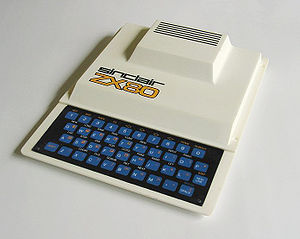
\includegraphics[width=0.5\textwidth]{ZX80}
	\end{figure}
	
	Nei corsi di Architettura degli Elaboratori negli anni 80 i processori studiati erano: il 6502 (8 bit, processore del computer Apple II, noto per essere stato costruito nel garage di Steve Jobs e Wozniak), Z80, processore a 16 bit del famoso computer ZX80 e l'Intel 8088. Tali processori raggiungevano al massimo una velocità di clock (detto molto a grandi linee, operazioni al secondo) dell'ordine di meno di una decina di MHz (Mega Hertz, milioni). I processori odierni raggiungono
	cicli di clock sull'ordine dei GHz (Giga Hertz, miliardi). Nel corso degli anni fino ad oggi, l'evoluzione dei processori ha seguito la \textbf{legge di Moore}. La "legge" spiega che ogni 18 mesi la potenza dei processori in commercio raddoppia, perché la densità dei transistor contenuti all'interno aumenta. Negli ultimi decenni abbiamo  miglioramenti architetturali come super pipeline e super scalari, ciò ha permesso di introdurre processori \textbf{multicore}, ovvero che contengono più "nuclei" interni (detti core) che elaborano le istruzioni dei processi in esecuzione in parallelo.
	Ad oggi il numero di core in uno smartphone raggiunge anche gli 8 core, mentre in processori per server sono stati raggiunti numeri di core anche intorno ai 64. I processori odierni utilizzano core a 64 bit, con architettura X86\_64 per Desktop o ARM per dispositivi mobili.
	Un componente fondamentale dell'evoluzione degli elaboratori è stato anche lo sviluppo dei processori grafici (GPU) con i quali ad oggi è possibile riprodurre grafica su schermo, ambienti tridimensionali molto complessi (videogiochi) o sfruttare la loro capacità di parallelizzazione per l'uso di reti neurali nell'intelligenza artificiale.
	
	Osserveremo i calcolatori a diversi livelli di \textbf{astrazione}
	
	I livelli di astrazione sono:
	\begin{itemize}
		\item Applicazioni utente
		\item Sistema Operativo
		\item Architettura (ASM, ad es. x86 o ARM)
		\item Microarchitettura
		\item Logica
		\item Circuiti digitali
		\item Device
		\item Fisica
	\end{itemize}
	
	Ogni livello si appoggia sul livello inferiore, ovvero è costruito sui componenti offerti dal livello inferiore. Dei principi fondamentali sono: \textbf{gerarchi, modularità e regolarità}
	
	La modularità è fondamentale per avere moduli organizzati gerarchicamente, autonomi ed indipendenti.
\end{note}



\begin{defn}
	\textbf{Set di Istruzioni}

	Distinguiamo due set di istruzioni dei processori, \textbf{CISC} e \textbf{RISC}. Gli acronimi sono rispettivamente \textbf{Complex Instruction Set Computer} e \textbf{Reduced Instruction Set Computer}, RISC contiene i processori ARM, che studieremo in dettaglio, mentre CISC comprende i processori più comuni nei desktop (X86 e X86\_64)
\end{defn}


\chapter{Rappresentazioni Numeriche e Testuali}

\section{Aritmetica Binaria}

I calcolatori utilizzano valori discreti (differenze di potenziale) fra 0 e 1 per rappresentare valori numerici. Viene detta Aritmetica Binaria l'aritmetica con i numeri rappresentati in base 2.

Siamo abituati a ragionare in base 10, ad esempio il numero 413 in base 10 è 
\[ 104 = 10^2 \cdot 1 + 10^1 \cdot 0 + 10^0 \cdot 4 \]

Lo stesso numero rappresentato in base 2 (codice binario) è

\[ 104_{10} = 01101000_2 = 2^7 \cdot 0 + 2^6 \cdot 1 + 2^5 \cdot 1 + 2^4 \cdot 0 + 2^3 \cdot 1 + 2^2 \cdot 0 + 2^1 \cdot 0 + 2^0 \cdot 0 \]

Un numero binario di 8 cifre è detto \textbf{byte}, un numero di 4 cifre è detto \textbf{nibble}. Una \textbf{parola} (\textbf{word}) è la quantità minima su cui viene rappresentato un intero in un calcolatore. Ad oggi le parole dei calcolatori sono 64 bit, alcuni calcolatori datati hanno parole da 32 bit.

La somma nell'aritmetica binaria è definita normalmente per i numeri positivi. Nei calcolatori i numeri hanno una dimensione finita (numero di bit) che indica il numero di cifre binarie con le quali è possibile rappresentare un numero. I positivi binari rappresentano numeri fino a $ 2^{N}-1 $ dove $ N $ è il numero di cifre.

Per rappresentare i numeri negativi si utilizza il metodo \textbf{segno-magnitudo} dove il bit più a sinistra rappresenta il segno (0 se il numero è positivo e 1 se è negativo). Il problema del metodo segno-magnitudo è che non rispetta la somma aritmetica. Può rappresentare numeri da $ [-2^{N-1}, +2^{N-1} ] $

Un metodo migliore per rappresentare i numeri negativi è il \textbf{complemento a due}. Nel complemento a due la cifra più a sinistra rappresenta sempre $ 2^{N-1} $ ma \textbf{negativo}. Il resto delle cifre sono positive e vengono sommate alla prima cifra negativa. Questo metodo rispetta la somma aritmetica. Per moltiplicare un numero per $ -1 $ si invertono le cifre binarie e si aggiunge 1 al numero. È possibile anche la sottrazione sommando un numero positivo ad uno negativo.

La somma fra due cifre può essere costruita con reti logiche. Il risultato della somma $ A + B = A \oplus B $ (operatore XOR) mentre il riporto della somma = $ A \land B $ (operatore AND)

\begin{figure}
	\centering
	\caption{Gate XOR}
	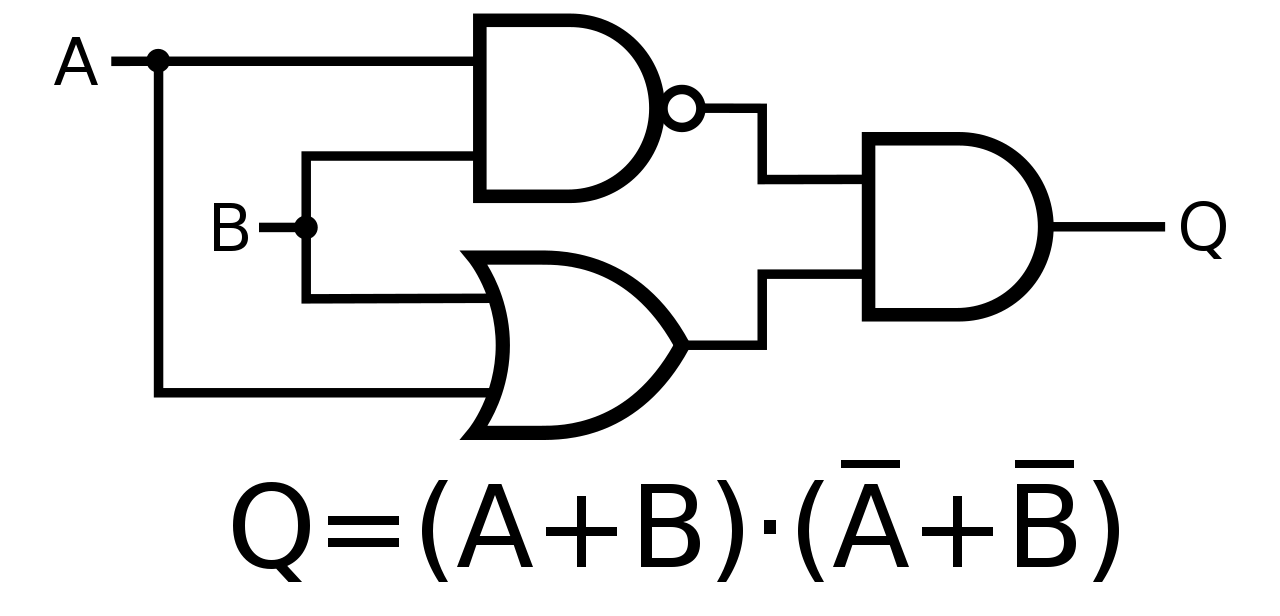
\includegraphics[width=\textwidth/2]{xor}
\end{figure}

\section{Esadecimale} 

I numeri esadecimali sono numeri in base 16. Siccome non bastano le cifre decimali per rappresentare i numeri maggiori di 9 si usano le prime lettere dell'alfabeto.
Una cifra esadecimale rappresenta un nibble (4 bit).

\section{Numeri in virgola mobile}

I numeri in virgola mobile si rappresentano con lo standard EEE 754 che definisce come si rappresentano i numeri in virgola mobile a singola precisione e doppia precisione (32 e 64 bit)

I bit del numero vengono divisi in 3 parti. Il primo bit denota il segno, la seconda parte rappresenta l'esponente e la terza parte si denota mantissa. L'esponente esprime dove la virgola verrà posizionata, come nella notazione scientifica di una calcolatrice l'esponente rappresenta $ 10^{n} $ dove $ n $ è l'esponente. La mantissa è un numero di base moltiplicato per $ 10^0 $, e viene successivamente moltiplicato per l'esponente.
L'esponente può essere sia positivo che negativo.

\begin{figure}
	\caption{Standard IEEE 754 a 32 bit}
	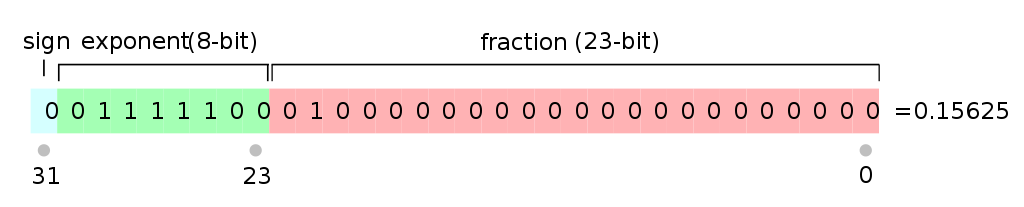
\includegraphics[width=\textwidth]{eee_floating_32}
\end{figure}

Nello standard a 32 bit la sezione esponente ha 8 bit di lunghezza. Un numero ad 8 bit può rappresentare numeri da 0 a 255, per ottenere gli esponenti negativi nello standard dei numeri a virgola mobile il numero a 8 bit rappresenta invece numeri da -127 a +128

\begin{figure}
	\caption{IEEE 754 a 64 bit}
	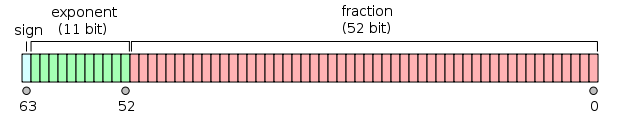
\includegraphics[width=\textwidth]{eee_floating_64}
\end{figure}

\paragraph{Somma dei numeri a virgola mobile}

Per sommare i numeri a virgola mobile il primo passo è allineare le mantisse, significa osservare gli esponenti e spostarli fino a che le cifre non sono sommabili in colonna.
Il secondo passo consiste nel sommare e il terzo passo nel normalizzare la somma. Nei processori la somma floating point viene eseguita in dei moduli appositi che in input ricevono due o più numeri floating point ed eseguono in dei sotto-moduli i tre passaggi della somma in un tempo $ 1/3 t $ dove $ t $ è il tempo totale per eseguire una somma. I tre passaggi della somma possono essere sequenzializzati così che una volta che ogni sotto-modulo ha completato il passo, può ricevere subito l'input successivo (la somma di due numeri FP impiegherà $ t + 1/3 $ invece che $ 2t $)

\paragraph{Estensioni vettoriali}
Alcuni processori permettono di eseguire operazioni contemporaneamente su un registro dividendolo in sottoregistri più piccoli. 

\section{Codifica ASCII}
La codifica ASCII è una tabella di codifica di caratteri testuali con interi da 0 a 255 (8 bit). La codifica ASCII estesa è a 16 bit e comprende diversi caratteri non latini.

\begin{figure}
	\caption{Tabella ASCII}
	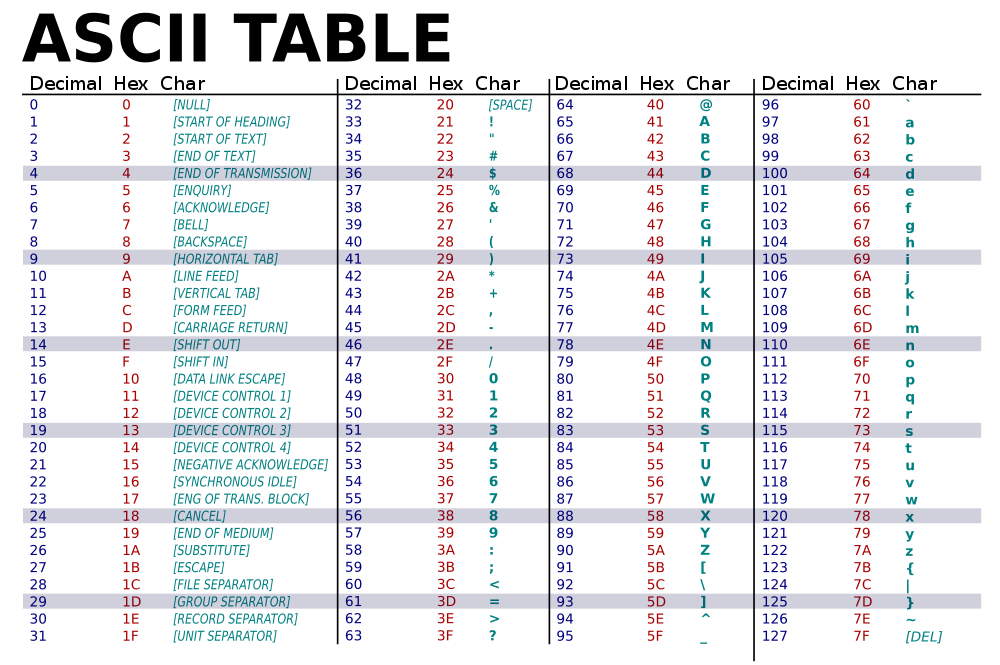
\includegraphics[width=\textwidth]{ascii}
\end{figure}

\section{Porte Logiche e Algebra di Boole}

I circuiti digitali vengono realizzati utilizzando componenti chiamati \textbf{porte logiche}. Sono realizzate con componenti fisici come transistor e resistenze, ma nella progettazione dei circuiti digitali le porte logiche vengono schematizzate con i simboli riportati nella Figura 3.1 per semplificare la progettazione \textbf{astraendo} il livello di complessità della circuiteria analogica.
Solamente con la porta NAND si possono realizzare tutte le altre porte (NAND è funzionalmente completo), ma le porte in generale si costruiscono singolarmente con componenti appositi. Esse implementano la \textbf{logica booleana} che conseguentemente permette di realizzare operazioni di \textbf{aritmetica binaria} per costruire unità di calcolo in componenti elettronici e processori.

\begin{wrapfigure}{r}{0.6\textwidth}
	\begin{center}
		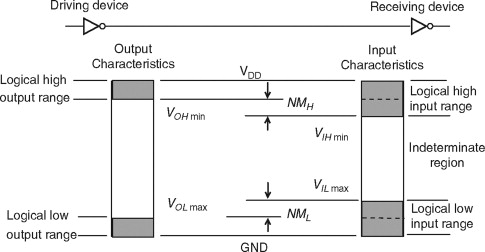
\includegraphics[width=0.58\textwidth]{noisemargin}
	\end{center}
	\caption{Margine di rumore nei circuiti digitali}	
\end{wrapfigure}


I componenti elettronici molto piccoli sono sensibili al \textbf{rumore}, per ovviare al problema i valori discreti (0 e 1) nei circuiti digitali non seguono un cambiamento istantaneo di differenza di potenziale (voltaggio), ma ammettono un margine per ridurre i problemi causati dal rumore.


I componenti (transistor) con cui si costruiscono porte logiche e circuiti sono realizzati con materiali semiconduttori, che possono essere di diversi tipi. Vedremo il tipo NMOS. Un transistor è composto da materiali come gallio e silicio.

\begin{wrapfigure}{r}{0.7\textwidth}
	\begin{center}
		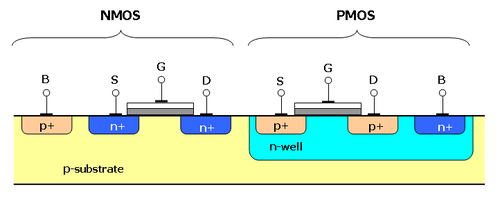
\includegraphics[width=0.68\textwidth]{cmos}
	\end{center}
	\caption{Transistor NMOS}
\end{wrapfigure}


\begin{figure}
	\centering
	\caption{Tabella delle porte logiche comuni}
	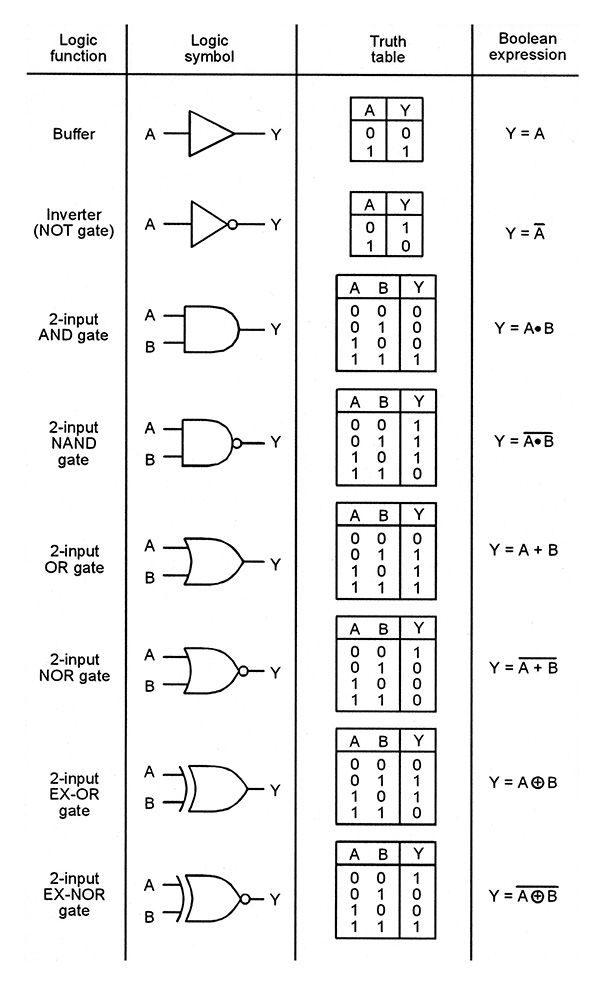
\includegraphics[width=\textwidth,height=\textheight]{logicgates}
\end{figure}

\begin{figure}
	\centering
	\caption{Porta NOT con transistor PMOS e NMOS}
	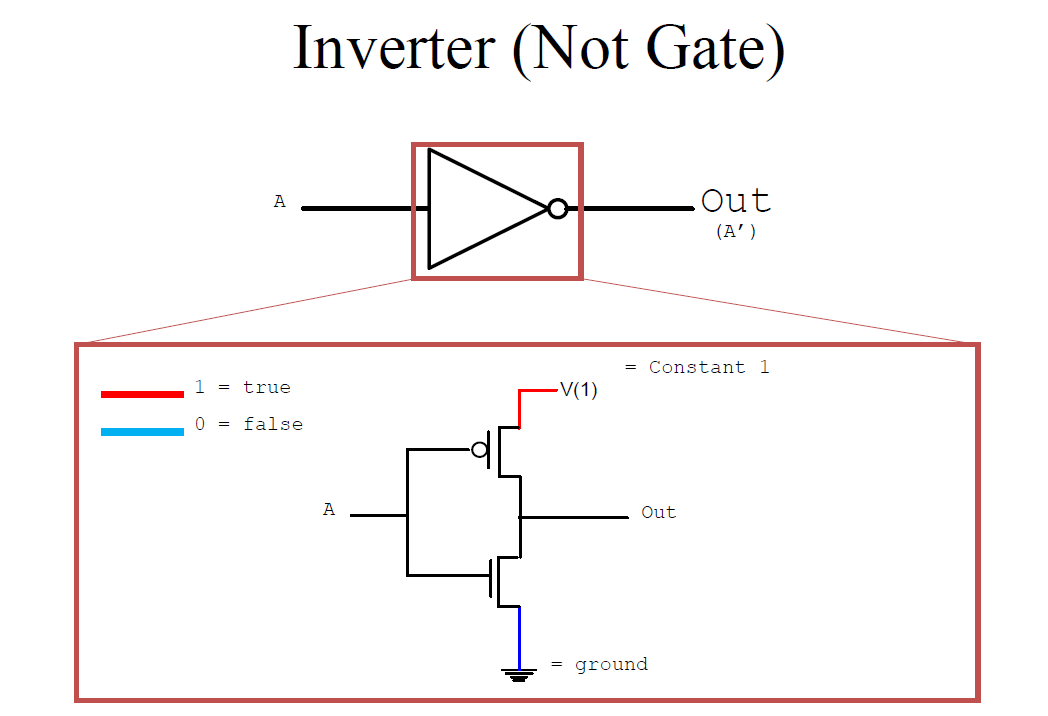
\includegraphics[width=\textwidth]{notgatetransistor}
\end{figure}

\begin{figure}
	\centering
	\caption{Transistor NMOS e PMOS}
	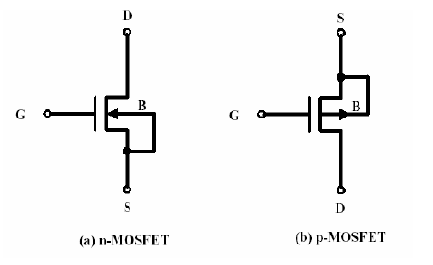
\includegraphics[width=0.6\textwidth]{NMOS-and-PMOS}
\end{figure}

\clearpage

\subsection{Algebra di Boole}


\begin{figure}[H]
	\centering
	
\includegraphics[width=0.48\textwidth]{sommadiprodotti-gate}
	\caption{Conversione di $ z $ da formula booleana a circuito logico}
\end{figure}

\begin{table}[H]
	\centering
	\caption{Notazione usata per l'Algebra di Boole}
	\label{tab:notazione-booleana}
	\begin{tabular}{|l|l|l|}
		\hline
		Funzione & Notazione Usata & Notazione Logica \\ 
		NOT(A)   & $\overbar{A}$   & $\lnot A$        \\ 
		AND(A,B) & $A \cdot B$     & $A \land B$      \\ 
		OR(A,B)  & $A + B$         & $A \lor B$       \\ \hline
	\end{tabular}
\end{table}

Prendiamo ad esempio un espressione booleana in forma canonica in \textbf{somma di prodotti}:
\[ z = \overbar{A}\overbar{B}\overbar{C} + \overbar{A}\overbar{B}C + \overbar{A}BC + A\overbar{B}C + ABC \]


\begin{table}[H]
	\centering
	\caption{Tabella di verità di $ z $}
	\label{tab:z-truth}
	\begin{tabular}{|l|l|l|l|}
		\hline
		A & B & C & z \\ \hline
		0                       & 0                      & 0 & 1 \\  
		0                       & 0                      & 1 & 1 \\ 
		0                       & 1                      & 0 & 0 \\ 
		0                       & 1                      & 1 & 1 \\ 
		1                       & 0                      & 0 & 0 \\ 
		1                       & 0                      & 1 & 1 \\  
		1                       & 1                      & 0 & 0 \\ 
		1                       & 1                      & 1 & 1 \\ \hline
	\end{tabular}
\end{table}




$ z $ si può anche esprimere come prodotto di somme: $ z = (A+\overbar{B}+C)(\overbar{A}BC)(\overbar{A}\overbar{B}C) $


\subsection{Teoremi dell'Algebra Booleana}
Breve ripasso dei teoremi della Logica Booleana.
\paragraph{Elemento Identità di prodotto e somma}
\[ A \cdot 1 = A \iff A \land T \equiv A\]
\[ A + 0 = 0 \iff A \lor F \equiv A\]
\paragraph{Elemento assorbente}
\[ A \cdot 0 = 0 \iff A \land F \equiv F \]
\[ A + 1 = 1 \iff A \lor T \equiv T \]
\paragraph{Idempotenza}
\[ A \cdot A = A \iff A \land A \equiv A \]
\[ A + A = A \iff A \lor A \equiv A \]
\paragraph{Complemento}
\[ A \cdot \overbar{A} = 0 \iff A \land \lnot A \equiv F \]
\[ A + \overbar{A} = 1 \iff A \lor \lnot A \equiv T \]
\paragraph{Commutatività}
\[ A + B = B + A \]
\[ A \cdot B = B \cdot A \]
\paragraph{Associatività}
\[ (A \cdot B) \cdot C = A \cdot (B \cdot C) \]
\[ (A + B) + C = A + (B + C) \]
\paragraph{Distributività}
\[ (A \cdot B) + C = (A+C) \cdot (B+C) \]
\[ (A+B) \cdot C = AC + BC \]
\paragraph{DeMorgan}
\[ \overbar{(A + B)} = \overbar{A} \cdot \overbar{B} \iff \lnot(A \lor B )\equiv \lnot A \land \lnot B \]
\[ \overbar{(A \cdot B)} = \overbar{A} + \overbar{B} \iff \lnot(A \land B )\equiv \lnot A \lor \lnot B \]

\paragraph{Esempio}
Semplifichiamo la formula booleana $ z = \overbar{A}\overbar{B}\overbar{C} + \overbar{A}\overbar{B}C + \overbar{A}BC + A\overbar{B}C + ABC $

\begin{align}
\begin{cases}
\overbar{A}\overbar{B}\overbar{C} + \overbar{A}\overbar{B}C \equiv \overbar{A}\overbar{B}(\overbar{C}+C) \equiv \overbar{A}\overbar{B} \\ 
A\overbar{B}C + ABC \equiv AC(\overbar{B}+B) \equiv AC
\end{cases} \\
\implies z = \overbar{A}\overbar{B} + \overbar{A}BC + AC
\end{align}

Le leggi della logica Booleana ci permettono di semplificare molto i componenti realizzati con porte logiche.

\subsection{Mappe di Karnaugh}

Una mappa di Karnaugh o K-Map è un metodo di semplificare un espressione booleana. I valori sono trasferiti da una tabella di verità ad una mappa bidimensionale:

Approfondisci su \href{https://en.wikipedia.org/wiki/Karnaugh_map}{Wikipedia}

Prendiamo una formula a quattro variabili $ f(A,B,C,D) $, una mappa di Karnaugh può essere:
\begin{table}[H]
	\centering
	\caption{Tabella di verità della mappa di Karnaugh di $f$}
	\label{tab:karnaugh}
	\begin{tabular}{lllll}
		AB\textbackslash{}CD    & 00                     & 01                     & 11                     & 10                     \\ \cline{2-5} 
		\multicolumn{1}{l|}{00} & \multicolumn{1}{l|}{1} & \multicolumn{1}{l|}{1} & \multicolumn{1}{l|}{1} & \multicolumn{1}{l|}{1} \\ \cline{2-5} 
		\multicolumn{1}{l|}{01} & \multicolumn{1}{l|}{1} & \multicolumn{1}{l|}{1} & \multicolumn{1}{l|}{0} & \multicolumn{1}{l|}{0} \\ \cline{2-5} 
		\multicolumn{1}{l|}{11} & \multicolumn{1}{l|}{0} & \multicolumn{1}{l|}{1} & \multicolumn{1}{l|}{0} & \multicolumn{1}{l|}{0} \\ \cline{2-5} 
		\multicolumn{1}{l|}{10} & \multicolumn{1}{l|}{0} & \multicolumn{1}{l|}{0} & \multicolumn{1}{l|}{1} & \multicolumn{1}{l|}{1} \\ \cline{2-5} 
	\end{tabular}
\end{table}

Facciamo ad esempio la mappa di Karnaugh di $ z = f(A,B,C) $ vista nella sezione precedente:

\begin{table}[H]
	\centering
	\caption{Tabella di verità della mappa di Karnaugh di $z$}
	\label{tab:karnaugh}
	\begin{tabular}{lllll}
		A\textbackslash{}BC    & 00                     & 01                     & 11                     & 10                     \\ \cline{2-5} 
		\multicolumn{1}{l|}{0} & \multicolumn{1}{l|}{1} & \multicolumn{1}{l|}{1} & \multicolumn{1}{l|}{1} & \multicolumn{1}{l|}{0} \\ \cline{2-5} 
		\multicolumn{1}{l|}{1} & \multicolumn{1}{l|}{0} & \multicolumn{1}{l|}{1} & \multicolumn{1}{l|}{1} & \multicolumn{1}{l|}{0} \\ \cline{2-5} 
	\end{tabular}
\end{table}

Possiamo riconoscere un'implicante nella seconda e terza colonna che corrisponde esattamente a C. Osserviamo un'altra implicante nella prima riga, prima e seconda colonna che corrisponde esattamente a $ \overbar{A}\overbar{B} $. Possiamo poi sommare le implicanti per ottenere una formula equivalente a quella di partenza, ciò implica che $ z =  \overbar{A}\overbar{B} + C $


\subsection{Circuito con più output}
Se abbiamo una tabella di verità di un circuito con $ n $ input e $ 2^n $ righe, con più output $ z_1, \dots, z_k $, gli output si suddividono in $ k $ tabelle con un solo output ($ z_k $) e $ 2^n $ righe di input.

\subsection{Operatori a più ingressi}
Gli operatori a più ingressi AND, OR, etc..., se presentano più di due ingressi si rappresentano con una rete logica che sfrutta la proprietà associativa degli operatori logici. Ciò comporta un limite massimo di ingressi perché viene introdotto un ritardo di stabilizzazione determinato e piccolo.
Ad esempio, un AND a 4 ingressi sarà rappresentato come $ z = x_1 \cdot x_2 \cdot x_3 \cdot x_4 = (x_1 \cdot x_2 ) \cdot (x_3 \cdot x_4)  $
Perciò gli operatori associativi a più ingressi si rappresentano come un albero k-ario di porte logiche. Il numero di livelli di porte sarà $ log_k(n) $ dove $ k $ è l'arietà delle singole porte ed è $ n $ il numero di ingressi nel circuito.

% TODO figura albero di AND con 8 input. 


\chapter{Porte Logiche e Algebra di Boole}

I circuiti digitali vengono realizzati utilizzando componenti chiamati \textbf{porte logiche}. Sono realizzate con componenti fisici come transistor e resistenze, ma nella progettazione dei circuiti digitali le porte logiche vengono schematizzate con i simboli riportati nella Figura 3.1 per semplificare la progettazione \textbf{astraendo} il livello di complessità della circuiteria analogica.
Solamente con la porta NAND si possono realizzare tutte le altre porte (NAND è funzionalmente completo), ma le porte in generale si costruiscono singolarmente con componenti appositi. Esse implementano la \textbf{logica booleana} che conseguentemente permette di realizzare operazioni di \textbf{aritmetica binaria} per costruire unità di calcolo in componenti elettronici e processori.

\begin{wrapfigure}{r}{0.6\textwidth}
	\begin{center}
		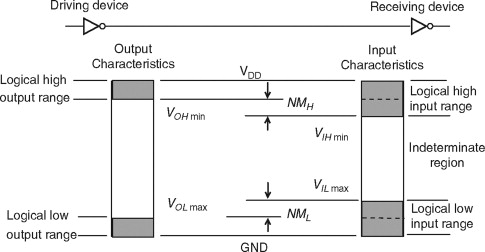
\includegraphics[width=0.58\textwidth]{noisemargin}
	\end{center}
	\caption{Margine di rumore nei circuiti digitali}	
\end{wrapfigure}


I componenti elettronici molto piccoli sono sensibili al \textbf{rumore}, per ovviare al problema i valori discreti (0 e 1) nei circuiti digitali non seguono un cambiamento istantaneo di differenza di potenziale (voltaggio), ma ammettono un margine per ridurre i problemi causati dal rumore.


I componenti (transistor) con cui si costruiscono porte logiche e circuiti sono realizzati con materiali semiconduttori, che possono essere di diversi tipi. Vedremo il tipo NMOS. Un transistor è composto da materiali come gallio e silicio.

\begin{wrapfigure}{r}{0.7\textwidth}
	\begin{center}
		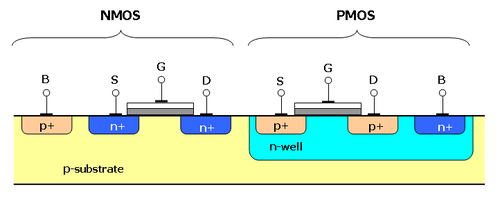
\includegraphics[width=0.68\textwidth]{cmos}
	\end{center}
	\caption{Transistor NMOS}
\end{wrapfigure}


\begin{figure}
	\centering
	\caption{Tabella delle porte logiche comuni}
	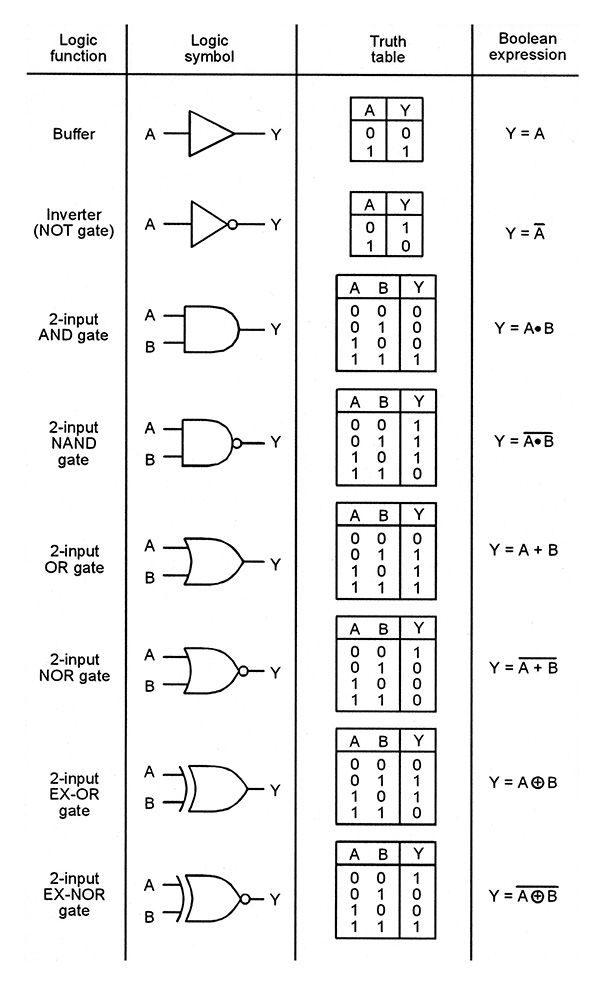
\includegraphics[width=\textwidth,height=\textheight]{logicgates}
\end{figure}

\begin{figure}
	\centering
	\caption{Porta NOT con transistor PMOS e NMOS}
	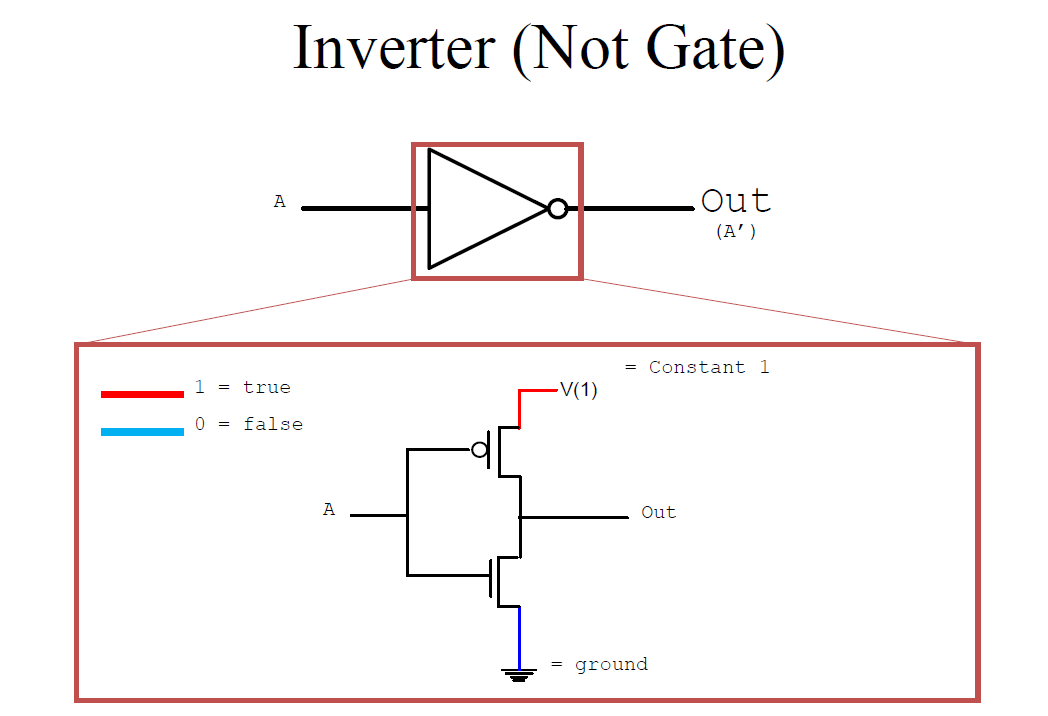
\includegraphics[width=\textwidth]{notgatetransistor}
\end{figure}

\begin{figure}
	\centering
	\caption{Transistor NMOS e PMOS}
	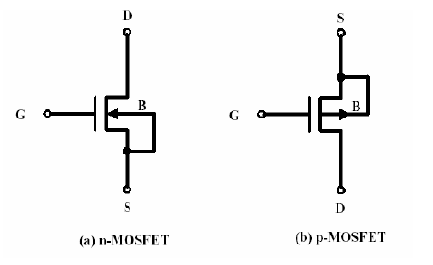
\includegraphics[width=0.6\textwidth]{NMOS-and-PMOS}
\end{figure}

\clearpage

% TODO porta logica NOT con MOS


\section{Algebra di Boole}

\begin{table}[H]
	\centering
	\caption{Notazione usata per l'Algebra di Boole}
	\label{tab:notazione-booleana}
	\begin{tabular}{|l|l|l|}
		\hline
		Funzione & Notazione Usata & Notazione Logica \\ 
		NOT(A)   & $\overbar{A}$   & $\lnot A$        \\ 
		AND(A,B) & $A \cdot B$     & $A \land B$      \\ 
		OR(A,B)  & $A + B$         & $A \lor B$       \\ \hline
	\end{tabular}
\end{table}

La forma canonica di espressioni booleane in \textbf{somma di prodotti} è:
\[ z = \overbar{A}\overbar{B}\overbar{C} + \overbar{A}\overbar{B}C + \overbar{A}BC + A\overbar{B}C + ABC \]

\begin{table}[H]
	\centering
	\caption{Tabella di verità di $ z $}
	\label{tab:z-truth}
	\begin{tabular}{|l|l|l|l|}
		\hline
		A & B & C & z \\ \hline
		0                       & 0                      & 0 & 1 \\  
		0                       & 0                      & 1 & 1 \\ 
		0                       & 1                      & 0 & 0 \\ 
		0                       & 1                      & 1 & 1 \\ 
		1                       & 0                      & 0 & 0 \\ 
		1                       & 0                      & 1 & 1 \\  
		1                       & 1                      & 0 & 0 \\ 
		1                       & 1                      & 1 & 1 \\ \hline
	\end{tabular}
\end{table}

$ z $ si può anche esprimere come prodotto di somme: $ z = (A+\overbar{B}+C)(\overbar{A}BC)(\overbar{A}\overbar{B}C) $

% TODO conversione da forma canonica somma di prodotti a circuito 4.3

\section{Teoremi dell'Algebra Booleana}
Breve ripasso dei teoremi della Logica Booleana.
\paragraph{Elemento Identità di prodotto e somma}
\[ A \cdot 1 = A \iff A \land T \equiv A\]
\[ A + 0 = 0 \iff A \lor F \equiv A\]
\paragraph{Elemento assorbente}
\[ A \cdot 0 = 0 \iff A \land F \equiv F \]
\[ A + 1 = 1 \iff A \lor T \equiv T \]
\paragraph{Idempotenza}
\[ A \cdot A = A \iff A \land A \equiv A \]
\[ A + A = A \iff A \lor A \equiv A \]
\paragraph{Complemento}
\[ A \cdot \overbar{A} = 0 \iff A \land \lnot A \equiv F \]
\[ A + \overbar{A} = 1 \iff A \lor \lnot A \equiv T \]
\paragraph{Commutatività}
\[ A + B = B + A \]
\[ A \cdot B = B \cdot A \]
\paragraph{Associatività}
\[ (A \cdot B) \cdot C = A \cdot (B \cdot C) \]
\[ (A + B) + C = A + (B + C) \]
\paragraph{Distributività}
\[ (A \cdot B) + C = (A+C) \cdot (B+C) \]
\[ (A+B) \cdot C = AC + BC \]
\paragraph{DeMorgan}
\[ \overbar{(A + B)} = \overbar{A} \cdot \overbar{B} \iff \lnot(A \lor B )\equiv \lnot A \land \lnot B \]
\[ \overbar{(A \cdot B)} = \overbar{A} + \overbar{B} \iff \lnot(A \land B )\equiv \lnot A \lor \lnot B \]

\paragraph{Esempio}
Semplifichiamo la formula booleana $ z = \overbar{A}\overbar{B}\overbar{C} + \overbar{A}\overbar{B}C + \overbar{A}BC + A\overbar{B}C + ABC $

\begin{align}
\begin{cases}
\overbar{A}\overbar{B}\overbar{C} + \overbar{A}\overbar{B}C \equiv \overbar{A}\overbar{B}(\overbar{C}+C) \equiv \overbar{A}\overbar{B} \\ 
A\overbar{B}C + ABC \equiv AC(\overbar{B}+B) \equiv AC
\end{cases} \\
\implies z = \overbar{A}\overbar{B} + \overbar{A}BC + AC
\end{align}

Le leggi della logica Booleana ci permettono di semplificare molto i componenti realizzati con porte logiche.

\section{Mappe di Karnaugh}

% TODO cos'è una mappa di Karnaugh

Prendiamo una formula a quattro variabili $ f(A,B,C,D) $, una mappa di Karnaugh può essere:
\begin{table}[H]
	\centering
	\caption{Tabella di verità della mappa di Karnaugh di $f$}
	\label{tab:karnaugh}
	\begin{tabular}{lllll}
		AB\textbackslash{}CD    & 00                     & 01                     & 11                     & 10                     \\ \cline{2-5} 
		\multicolumn{1}{l|}{00} & \multicolumn{1}{l|}{1} & \multicolumn{1}{l|}{1} & \multicolumn{1}{l|}{1} & \multicolumn{1}{l|}{1} \\ \cline{2-5} 
		\multicolumn{1}{l|}{01} & \multicolumn{1}{l|}{1} & \multicolumn{1}{l|}{1} & \multicolumn{1}{l|}{0} & \multicolumn{1}{l|}{0} \\ \cline{2-5} 
		\multicolumn{1}{l|}{11} & \multicolumn{1}{l|}{0} & \multicolumn{1}{l|}{1} & \multicolumn{1}{l|}{0} & \multicolumn{1}{l|}{0} \\ \cline{2-5} 
		\multicolumn{1}{l|}{10} & \multicolumn{1}{l|}{0} & \multicolumn{1}{l|}{0} & \multicolumn{1}{l|}{1} & \multicolumn{1}{l|}{1} \\ \cline{2-5} 
	\end{tabular}
\end{table}

Facciamo ad esempio la mappa di Karnaugh di $ z = f(A,B,C) $ vista nella sezione precedente:

\begin{table}[H]
	\centering
	\caption{Tabella di verità della mappa di Karnaugh di $z$}
	\label{tab:karnaugh}
	\begin{tabular}{lllll}
		A\textbackslash{}BC    & 00                     & 01                     & 11                     & 10                     \\ \cline{2-5} 
		\multicolumn{1}{l|}{0} & \multicolumn{1}{l|}{1} & \multicolumn{1}{l|}{1} & \multicolumn{1}{l|}{1} & \multicolumn{1}{l|}{0} \\ \cline{2-5} 
		\multicolumn{1}{l|}{1} & \multicolumn{1}{l|}{0} & \multicolumn{1}{l|}{1} & \multicolumn{1}{l|}{1} & \multicolumn{1}{l|}{0} \\ \cline{2-5} 
	\end{tabular}
\end{table}

Possiamo riconoscere un'implicante nella seconda e terza colonna che corrisponde esattamente a C. Osserviamo un'altra implicante nella prima riga, prima e seconda colonna che corrisponde esattamente a $ \overbar{A}\overbar{B} $. Possiamo poi sommare le implicanti per ottenere una formula equivalente a quella di partenza, ciò implica che $ z =  \overbar{A}\overbar{B} + C $


\subsection{Circuito con più output}
Se abbiamo una tabella di verità di un circuito con $ n $ input e $ 2^n $ righe, con più output $ z_1, \dots, z_k $
\chapter{Reti Sequenziali, Verilog e RTL}

Gli RTL, o Register Transfer Language, permettono di descrivere cosa succede a livello di circuito fra registri. Vengono utilizzati per descrivere l'hardware. Vedremo il linguaggio \textbf{Verilog}. Gli RTL permettono di descrivere e comporre dei moduli. Il libro di testo propone il dialetto \textbf{System Verilog} che mette a disposizione due metodi per descrivere i moduli. Un metodo è il metodo \textit{constructive}, noi vedremo il metodo \textit{behavioral} dove ad esempio un Multiplexer da 2 vie 1 bit è descritto da:
\begin{lstlisting}[style={verilog}]
	z = (ic == 0 ? x : y)
\end{lstlisting}

Verilog è un linguaggio compilato. Un file System Verilog compilato produce una traccia di esecuzione e un eseguibile che simula il comportamento dei moduli. Viene detta \textbf{simulazione}.

Un programma Verilog può anche essere dato in input a un programma detto \textbf{synthetizer}, che produce una \textbf{netlist}, ovvero una lista dei componenti e dei collegamenti per realizzare il modulo fisicamente. Un altro modo per realizzare la sintesi è utilizzare un \textbf{FPGA}, o Field-programmable gate array. Un FPGA è un circuito integrato composto da una matrice di celle, e una singola cella può:
\begin{enumerate}
	\item Eseguire una funzione booleana di 3-5 ingressi con 1 uscita 
	\item Implementare un bit di memoria
	\item Routing
\end{enumerate} 

Un FPGA moderno comprende, oltre a delle celle, delle righe che contengono diversi componenti come delle ALU.

\begin{figure}[H]
	\centering
	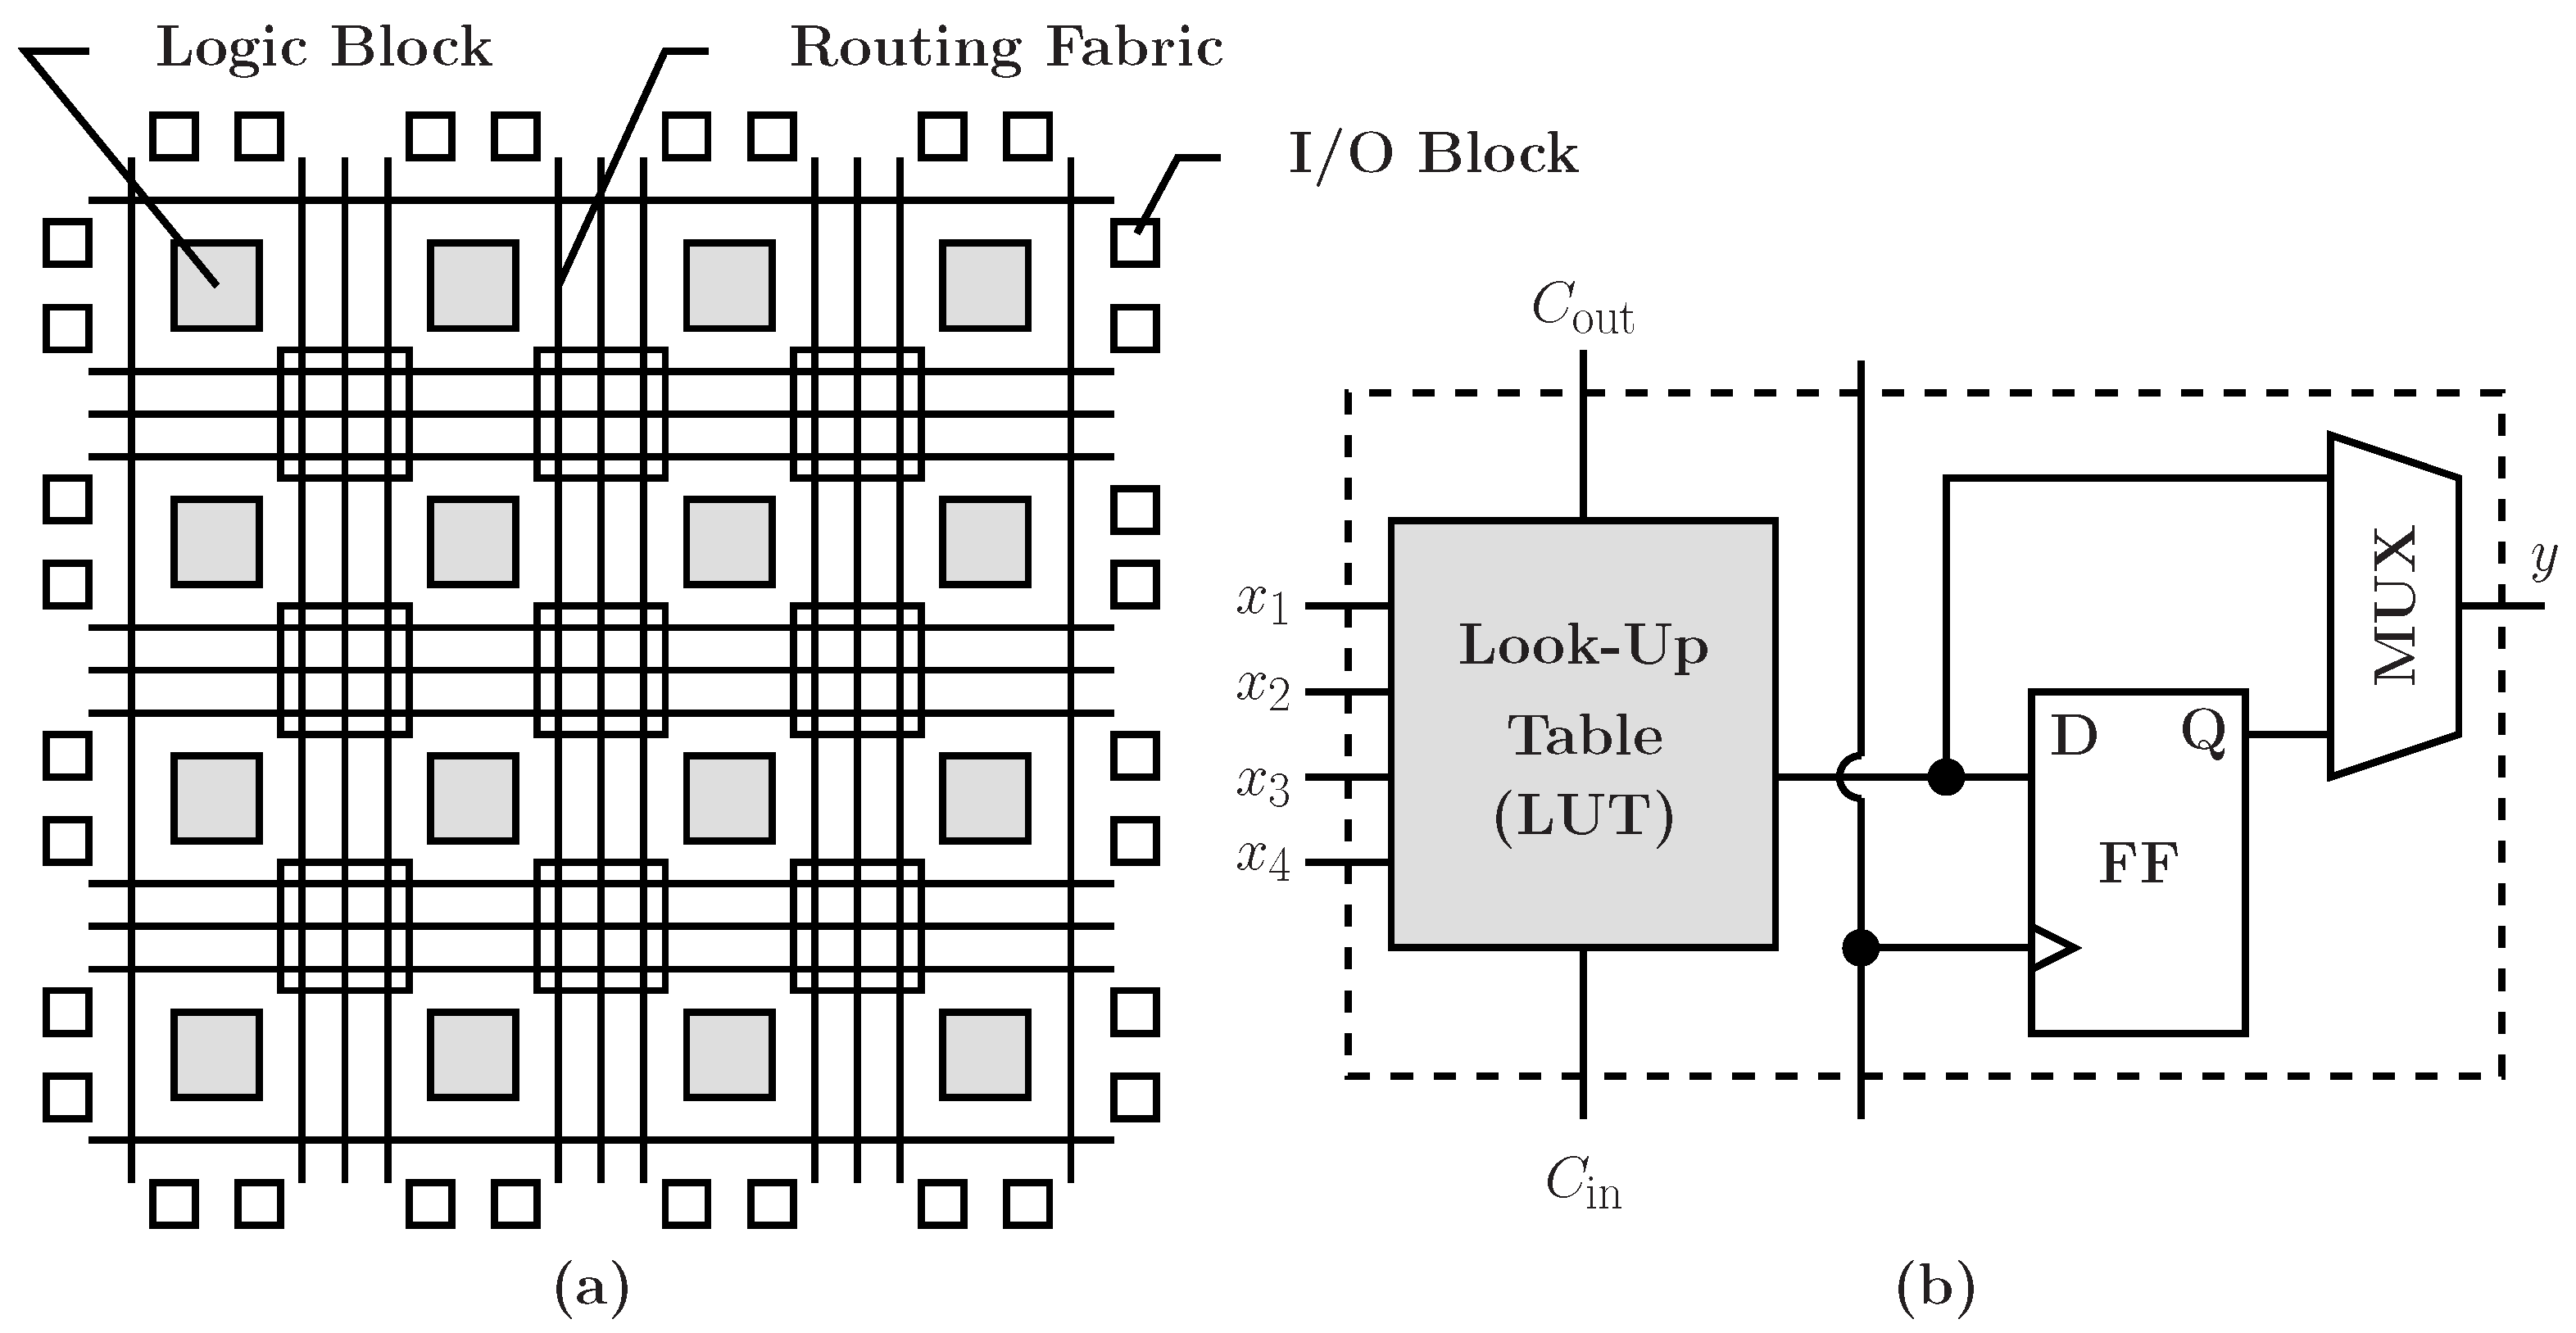
\includegraphics[]{fpga1}
	\caption{Schema FPGA}
\end{figure}

\section{Scrivere e compilare System Verilog}

Creiamo un multiplexer da due bit con System Verilog, compiliamo e visualizziamo con \textbf{GTKWave}

\includecode[verilog]{./verilog/2x1mux/mux.sv}{mux.sv}
\includecode[verilog]{./verilog/2x1mux/test_mux.sv}{test\_mux.sv}

Per compilare, eseguiamo da terminale 
\begin{lstlisting}[style={bash}]
iverilog -g2005-sv nome_sorgente.sv -o nome_eseguibile
\end{lstlisting}

Quindi, per compilare entrambi i file e caricarli in GTKWave:
\begin{lstlisting}[style={bash}]
iverilog -g2005-sv test_mux.sv mux.sv -o test_mux
# Eseguiamo la simulazione
./test_mux
# Viene creato il file provamux.vcd, carichiamolo in GTKWave
gtkwave provamux.vcd &
\end{lstlisting}

\includecode[verilog]{./verilog/2x1mux/mux4.sv}{Multiplexer da 4 vie ad 1 bit}

\includecode[verilog]{./verilog/2x1mux/muxbool.sv}{Multiplexer di variabili booleane}

\clearpage

\section{Esercizi}
\subsection{Automa che riconosce "abba"}

Realizziamo un automa di Mealy che riconosce le stringhe \textit{"abba"} da un insieme $ \{a,b,c\} $. La rete sequenziale dell'automa si realizzerà con i componenti visti in figura ~\ref{fig:mealyautomata1.tex}. Consideriamo la rappresentazione binaria dell'alfabeto con $ a = 00, b = 01, c = 11 $. Per gli stati usiamo la codifica $ S_1 = 00, S_2 = 01, S_3 = 11, S_4 = 10 $

\begin{figure}[H]
	\centering
	\caption{Automa di Mealy che riconosce "abba"}
	\begin{tikzpicture}[->,>=stealth',shorten >=1pt,auto,node distance=3.5cm]
	
	\node[state,accepting] 	(A)                    {$S_1$};
	\node[state]         	(B) [above right of=A] 	   {$S_2$};
	\node[state]         	(C) [below right of=B] 	   {$S_3$};
	\node[state]         	(D) [below right of=A] 	   {$S_4$};
	
	\path 	(A)		edge [bend left]  	node {$a/0$} 		(B)
	edge [loop left] 	node {$b,c/0$} 		(A)
	(B) 	edge [loop above] 	node {$a/0$} 		(B)
	edge [bend left] 	node {$c/0$} 		(A)
	edge [bend left]  	node {$b/0$} 		(C)
	(C)		edge [bend left]  	node {$c/0$} 		(A)
	edge [bend left]  	node {$a/0$} 		(B)
	edge [bend left]  	node {$b/0$} 		(D)
	(D)		edge [bend left]  	node {$b,c/0$} 		(A);
	\end{tikzpicture}
\end{figure}

\begin{table}[H]
	\centering
	\caption{Tabella di verità dell'output della rete sequenziale dell'automa "abba" ($ \omega $)}
	\label{tab:mealyomega2}
	\begin{tabular}{l|llll|l|}
		\cline{2-6}
		& $s_1$ & $s_2$ & $x_1$ & $x_2$ & z \\ \cline{2-6} 
		Stato $S_1$ & 0     & 0     & -     & -     & 0 \\
		Stato $S_2$ & 0     & 1     & -     & -     & 0 \\
		Stato $S_3$ & 1     & 1     & -     & -     & 0 \\
		Stato $S_4$ & 1     & 0     & 0     & 0     & 1 \\
		& 1     & 0     & 0     & 1     & 0 \\
		& 1     & 0     & 1     & 1     & 0 \\ \cline{2-6} 
	\end{tabular}
\end{table}

\begin{table}[H]
	\centering
	\caption{Tabella di verità del cambio di stato dell'automa per riconoscere "abba" ($\sigma$)}
	\label{tab:mealysigma2}
	\begin{tabular}{l|llll|ll|}
		\cline{2-7}
		& $s_1$ & $s_2$ & $x_1$ & $x_2$ & $s_1'$ & $s_2'$ \\ \cline{2-7} 
		Stato $S_1$ & 0     & 0     & 0     & 0     & 0      & 1      \\
		& 0     & 0     & 0     & 1     & 0      & 0      \\
		& 0     & 0     & 1     & 1     & 0      & 0      \\ \cline{2-7} 
		Stato $S_2$ & 0     & 1     & 0     & 0     & 0      & 1      \\
		& 0     & 1     & 0     & 1     & 1      & 1      \\
		& 0     & 1     & 1     & 1     & 0      & 0      \\ \cline{2-7} 
		Stato $S_3$ & 1     & 1     & 0     & 0     & 0      & 1      \\
		& 1     & 1     & 0     & 1     & 1      & 0      \\
		& 1     & 1     & 1     & 1     & 0      & 0      \\ \cline{2-7} 
		Stato $S_4$ & 1     & 0     & 0     & 0     & 0      & 0      \\
		& 1     & 0     & 0     & 1     & 0      & 0      \\
		& 1     & 0     & 1     & 1     & 0      & 0      \\ \cline{2-7} 
	\end{tabular}
\end{table}

% TODO mappa di karnaugh di s1 e s2

Avremo che la formula booleana sarà per il primo e secondo bit di stato:
\[ s_1' = \overbar{s_1}s_2\overbar{x_1}x_2 + s_1s_2\overbar{x_1}x_2 = s_2\overbar{x_1}x_2 \]. 
\[ s_2' = \overbar{s_1s_2}+ \overbar{s_1}s_2\overbar{x_1} + s_2\overbar{x_2}\]

La formula per l'uscita sarà $ z = s_1\overbar{s_2x_1x_2} $. Ci rimane da definire il registro da 2 bit per definire tutta la rete sequenziale. Abbiamo supposto che la rete sequenziale funzioni ricevendo un segnale di clock ad intervalli regolari.
La rete di output $ \omega $ è definita utilizzando soltanto AND ed impiegherà $ \Delta t $ per eseguire l'operazione. La funzione di cambio di stato $ \sigma $ è definita invece con 1 AND e 1 OR ed impiegherà $ 2\Delta t $ per l'operazione.
Il ciclo di clock dev'essere almeno $ \tau = \delta + \max\{t_{\sigma}, t_{\omega}\} $ dove $ \delta $ è la durata del segnale HIGH nel clock.

Abbiamo 3 moduli. Uno per il registro, uno per il modulo $ \omega $ e uno per il modulo $ \sigma $. Scriviamolo in Verilog.

\paragraph{Note}

La sintassi \verb|[a:b]| denota un array indicizzato dal numero \verb|a| al numero \verb|b|. Utilizziamo gli array per rappresentare valori a più bit. In questo caso, il registro è generalizzato per un parametro \verb|N| e può ad esempio essere inizializzato con \verb|registro #(4) nome(...) | dove 4 è il parametro \verb|N| e corrisponde al numero di bit del registro.

La negazione con \verb|!| nega un singolo valore, mentre la notazione \verb|~| viene detta negazione \textit{bit wise} e nega tutti i valori di una sequenza di bit.

Normalmente, in un blocco \verb|assign| assegno un valore ad una variabile booleana istantaneamente. Posso invece aggiungere un delay inserendo \verb|#x| di fronte all'identificatore della variabile, dove \verb|x| è un numero. Ad esempio:
\begin{lstlisting}[style={verilog}]
assign 
	#1 z = (ic == 0 ? x : y)
\end{lstlisting}

\includecode[verilog]{./verilog/abba/Registro/reg.v}{Registro a N bit}
\includecode[verilog]{./verilog/abba/Mealy/sigma.v}{Modulo di $ \sigma $ o funzione di cambio di stato}
\includecode[verilog]{./verilog/abba/Mealy/omega.v}{Modulo di $ \omega $}
\includecode[verilog]{./verilog/abba/Mealy/m1.v}{Modulo della rete sequenziale}
\includecode[verilog]{./verilog/abba/Mealy/test-m1.v}{Modulo di test della rete sequenziale}

\clearpage

\subsection{Automa di Moore per riconoscere "abba"}
Vediamo adesso un automa di Moore per riconoscere la stringa \textit{"abba"} nell'alfabeto $ \{a,b,c\} $. La differenza sta nel fatto che i singoli nodi non hanno accesso all'input $ x $.

\begin{figure}
	\centering
	\caption{Automa di Moore che riconosce "abba"}
	\begin{tikzpicture}[->,>=stealth',shorten >=1pt,auto,node distance=3.5cm]
	
	\node[state,initial] 	(A)                    {$\dfrac{S_1}{0}$};
	\node[state]         	(B) [right of=A] 	   {$\dfrac{S_2}{0}$};
	\node[state]         	(C) [below of=A] 	   {$\dfrac{S_3}{0}$};
	\node[state]         	(D) [below of=B] 	   {$\dfrac{S_4}{0}$};
	\node[state,accepting]  (E) [above right of=D] 	   {$\dfrac{S_4}{0}$};
	
	\path 	(A)		edge [bend left=60]  				node {$a$} 		(B)
					edge [loop above] 					node {$b,c$} 	(A)
			(B) 	edge [loop above] 					node {$a$} 		(B)
					edge [] 							node {$c$} 		(A)
					edge [bend left=20]  				node {$b$} 		(C)
			(C)		edge []  							node {$c$} 		(A)
					edge [bend left=20]  				node {$a$} 		(B)
					edge []  							node {$b$} 		(D)
			(D)		edge [bend left=90,looseness=2]		node {$b,c$} 	(A)
					edge []								node {$a$}		(E)
			(E)		edge [bend right=90,looseness=1.8]  	node {$b,c$} 	(A)
					edge []	node {$a$}		(B);
	\end{tikzpicture}
\end{figure}

\includecode[verilog]{./verilog/abba/Moore/mo-sigma.v}{Modulo di $ \sigma $ o funzione di cambio di stato (Moore)}
\includecode[verilog]{./verilog/abba/Moore/mo-omega.v}{Modulo di $ \omega $ (Moore)}
\includecode[verilog]{./verilog/abba/Moore/moore.v}{Modulo della rete sequenziale (Moore)}
\includecode[verilog]{./verilog/abba/Moore/test-m1.v}{Modulo di test della rete sequenziale (Moore)}
\includecode[makefile]{./verilog/abba/Moore/makefile}{Makefile (Moore)}

\FloatBarrier

\subsection{Mealy con Delay $ \equiv $ Moore}

\includecode[verilog]{./verilog/abba/MealyConDelay/reg-delay.v}{Registro a N bit con delay}
\includecode[verilog]{./verilog/abba/MealyConDelay/sigma-delay.v}{Modulo di $ \sigma $ o funzione di cambio di stato (Mealy con Delay)}
\includecode[verilog]{./verilog/abba/MealyConDelay/omega-delay.v}{Modulo di $ \omega $ (Mealy con Delay)}
\includecode[verilog]{./verilog/abba/MealyConDelay/m1-delay.v}{Modulo della rete sequenziale (Mealy con Delay)}
\includecode[verilog]{./verilog/abba/MealyConDelay/test-m1-delay.v}{Modulo di test della rete sequenziale (Mealy con Delay)}
\includecode[makefile]{./verilog/abba/MealyConDelay/makefile}{Makefile (Mealy con Delay)}

Per sincronizzare il modulo della rete sequenziale dell'automa di Mealy mettiamo un registro di fra l'input \verb|x| e le reti sequenziali \verb|sigma| e \verb|omega|
\chapter{Memorie e Parallelismo}

\section{Memorie}
Un componente fondamentale di un processore è la \textbf{memoria}. Si implementa utilizzando dei registri da $ n $ bit (dette parole). Vogliamo realizzare una memoria il cui accesso sia simile ad un array nel linguaggio C. Ovvero vogliamo avere un vettore di registri a cui possiamo accedere con un offset intero. Data una memoria $ A $ si accederà alla parola $ k-esima $ tramite $ A[k] $. Per implementare tale selezione si può utilizzare un multiplexer che riceve in input le uscite dei singoli registri. I singoli registri ricevono tutti un segnale di clock in input, e permettono la scrittura attraverso un demultiplexer (decoder) che dato un indirizzo invia un 1 all'enable del registro selezionato. Si può mettere in AND il segnale enable del decoder insieme ad un input enable generale.

L'implementazione reale delle memorie (in particolare memorie flash), avviene ponendo delle linee dette "di parola" (orizzontali) e linee dette "bit line" (verticali) in una matrice.
All'incrocio delle linee vi è un condensatore. Il condensatore mantiene una carica per un breve periodo di tempo. Ho modo di controllare se nel condensatore alla posizione $ xy $ era "ricordato" un valore 1, mandando della corrente lungo la "linea di parola" $ x $. Se il condensatore era carico esso si scarica lungo la linea "bit line" $ y $. Inviando della corrente sulla linea di parola $ x $ leggeremo quindi dalle bit line (in alcuni casi indicate come source lines in output) la parola $ x $.
Prima di un condensatore, si inserisce un transistor nella giunzione fra WL e BL. Utilizzando un condensatore, nelle RAM dinamiche (Dynamic Random Access Memory) possono insorgere problemi dovuti ai tempi di carica e scarica del condensatore. Una volta letto un valore su una Bit Line, il condensatore si scarica e "perde" il valore precedentemente "ricordato".

\centerfig{0.65}{flashmem}{Memoria Flash}

Per selezionare la Word Line utilizziamo sempre un demultiplexer (decoder) che riceve un indirizzo. Nelle ram DDR comuni sono presenti spesso 8 o 9 chip. Ad esempio, su uno stick di ram DDR3 da 1GB (1 Giga Byte) sono presenti 8 memorie da 1Gb (1 Giga Bit), e generalmente anche una nona memoria che ricorda la "parità" per il controllo degli errori. Le RAM dinamiche perdono il loro contenuto se non sono alimentate. Visto il comportamento dei condensatori (la loro carica si perde lentamente) le DRAM hanno bisogno di un \textbf{refresh} periodico. Le DRAM sono molto economiche (1 transistor per 1 bit) ma possono risultare più lente rispetto alle alternative SRAM. Le memorie SRAM (Static RAM) sono meno economiche ma più rapide rispetto alle DRAM. Utilizzano flip-flop invece dei condensatori e per ogni bit utilizzano 6 transistor. Le memorie all'interno del processore (calcolatore) sono memorie statiche (realizzate con flip-flop) molto rapide. Un meccanismo sia a livello hardware che a livello di S.O. permette la suddivisione dei dati processati fra vari livelli di cache, dalla memoria statica del processore alla più capiente ma lenta DRAM.

\centerfig{0.35}{dramcell}{Schema di una cella di una memoria DRAM}

\begin{defn}
	\textbf{RAM, ROM, PROM e EEPROM:}
	L'acronimo RAM (Random Access Memory) indica in generale delle memorie sulle quali possiamo leggere e scrivere. Le memorie ROM sono memorie a sola lettura (Read Only Memory). Le memorie ROM non hanno condensatori nelle giunzioni della matrice, ma a momento di produzione vengono "incisi" dei collegamenti o isolamenti nelle giunzioni fra Word Line e Bit Line.
	Le memorie \textbf{PROM} utilizzano dei fusibili nelle giunzioni fra WL e BL per permettere agli acquirenti di scrivere nella memoria una volta sola. Di fabbrica tutti i bit di una PROM sono impostati a 1. Bruciando i fusibili nelle giunzioni si interrompono i collegamenti realizzando una vera e propria scrittura permanente. 
	
	\centerfig{0.65}{prom}{Esempio di memoria PROM}
	
	Un altro tipo di memorie sono le \textbf{EEPROM} (Electrically Erasable ROM). Utilizzano dei transistor particolari che possono essere "reimpostati" permettendo di cancellare e riscrivere la memoria con una corrente maggiore.
	
	Nella seconda parte del corso vedremo dettagliatamente Assembly ARM. Le istruzioni Assembly eseguono delle operazioni sui registri interni alla CPU.
	Un esempio di istruzione banale è la somma di numeri fra registri. \verb|ADD R1 R2 R3|. Nell'Assembly ARM la lettura avviene da destra a sinistra, ed il risultato viene memorizzato nel registro più a sinistra, in questo caso \verb|R1|.	
\end{defn}



\paragraph{Memorie Multi Porta e Tempi di Accesso}
Le memorie multiporta permettono la lettura parallela di due o più registri. Invece di un singolo multiplexer per leggere un registro, alle uscite dei registri è collegato un altro multiplexer che ricevendo un indirizzo diverso dal primo multiplexer, permette di leggere un altro valore dalla memoria, abilitando alla lettura parallela di due registri contemporaneamente. È fondamentale avere una memoria con almeno due porte per eseguire istruzioni su due registri alla volta. Indichiamo i tempi di accesso alla memoria con $ T_a $. Ad oggi siamo in un range di tempi inferiori ad un nanosecondo per i tempi di accesso ai flip-flop (poche decine di picosecondi), sull'ordine dei nanosecondi per le SRAM (cache) e sull'ordine dei microsecondi per le DRAM.


\centerfig{0.75}{DRAM512}{Modulo RAM Corsair DDR2-533}

\paragraph{Blocco memoria}
Introduciamo un blocco per la memoria da utilizzare nei diagrammi dei circuiti.
La memoria riceve in input un dato $ x $ da scrivere nell'indirizzo indicato dall'input di controllo \textbf{Address}. Se il segnale \textbf{enable} è HIGH allora avviene la scrittura di $ x $ all'interno dell'indirizzo puntato. Altrimenti, se \textbf{enable} è LOW avviene la lettura. Assumiamo che l'uscita sia stabile per il ciclo di clock
\diagram{memoryblock.tex}{Blocco Memoria}

\paragraph{LUT (Lookup Table)}
Una rete combinatoria che riceve $ n $ bit in input può essere implementata con una memoria ROM. Data una tabella di verità di una rete combinatoria, si può portare la tabella di verità in forma vettoriale per creare una LUT.
Una LUT o \textbf{Lookup Table} è in generale un array che rimpiazza una computazione, possibilmente complessa, con un operazione di accesso, nel caso delle reti combinatorie con una memoria ROM.
I bit in input della tabella di verità vengono portati a bit rappresentanti l'indirizzo di accesso della memoria, e i risultati della tabella di verità saranno memorizzati in un vettore di $ 2^n $ elementi (se la tabella di verità ha un solo output). 
Per quanto alcune reti combinatorie possono risultare più complesse a livello di circuito se implementate con una LUT, un vantaggio non banale delle Lookup Tables è che possono essere riprogrammate se viene utilizzata una memoria EEPROM. Ciò svolge un ruolo fondamentale negli FPGA. Le LUT possono essere utilizzate in parallelo.

\begin{exmp}
	\textbf{Rete Sequenziale di un contatore}
	Se volessimo realizzare un contatore, con le sole operazioni di incremento e decremento con un ASF, dovremmo avere un numero di stati pari alla capacità massima del contatore.
	Per realizzare un contatore sono necessari un registro da $ n $ bit, (prendiamo ad esempio 8 bit) ed una ALU che fa due sole operazioni (+1 e -1), quindi con un solo bit di controllo. Scegliamo se aumentare o decrementare il contatore impostando il bit di controllo della ALU, e scegliamo se scrivere nel prossimo ciclo di clock impostando ad HIGH il bit Enable (Event) del registro. Essendo una rete sequenziale, la funzione $ \sigma $ è implementata dalla ALU, e la funzione $ \omega $ è semplicemente l'identità. È una rete di Moore poiché la funzione identità non dipende dagli ingressi (Inc/Dec ed Event).
	
	\diagram{counter.tex}{Rete sequenziale di un contatore}
\end{exmp}


\begin{exmp}
	\textbf{Semplice Calcolatrice}
	Vogliamo realizzare una calcolatrice molto semplice da 32 bit per eseguire addizione, sottrazione, moltiplicazione e divisione. La calcolatrice riceverà in input due numeri $ A,B $ e restituirà in output il risultato, che potrà essere re-inserito nei due registri contenenti $ A $ e $ B $. Essa è una rete sequenziale che possiamo inserire in un componente che avrà in input i due numeri $ A,B $, la selezione dei due multiplexer per gli input, segnali di enable per la scrittura nel registro $ A $ e nel registro $ B $ e due bit di controllo per selezionare l'operazione. In output avrà il numero in uscita e 4 bit di flag (Overflow, Carry, Negative e Zero). Definiamo questa parte del calcolatore "parte operativa". Abbiamo bisogno anche di una "parte di controllo" che dati due input si occuperà di controllare le entrate di controllo della parte operativa della calcolatrice.
	
	\diagram{calculator.tex}{Semplice Calcolatore (Omesso clock per semplicità del disegno, è presente)}
\end{exmp}


\begin{defn}
	\textbf{if-then-else:}
	Supponiamo di voler realizzare un importante costrutto per la programmazione (\textit{if-then-else}) utilizzando solo componenti standard. Abbiamo due reti combinatorie $ f,g $, una parola memorizzata in un registro $ A $ e un registro $ B $ in cui sarà memorizzato il risultato. Vogliamo costruire una rete per evaluare l'espressione:
	
	\begin{Verbatim}
	if(expr) then
		g(A) -> B
	else
		f(A) -> B
	\end{Verbatim}
	
	\diagram{ifthenelse.tex}{Rete che implementa if-then-else}
\end{defn}

\begin{defn}
	\textbf{while:}
	Se volessimo invece implementare un ciclo while della forma:
	\begin{Verbatim}
	while(expr) do
	f(A) -> A
	\end{Verbatim}
	Possiamo realizzarlo con la seguente rete:
	
	\diagram{while.tex}{Rete che implementa while}
	
	In maniera simile è possibile realizzare anche un costrutto switch-case.
	Icarus Verilog, per trasformare programmi Verilog di moduli behavioural in netlist di componenti di reti logiche utilizza meccanismi simili.
\end{defn}

\begin{exrc}
	\textbf{Confronto maggiore}
	
	Vediamo ora diversi metodi per realizzare una rete combinatoria che controlla se un numero è maggiore di un altro, utile per realizzare operazioni condizionali.
	
	\includecode[verilog]{./verilog/confrontomaggiore/maggioreb.v}{Esercizio di confronto maggiore in Verilog (approccio algoritmico)}
	
	\FloatBarrier	
\end{exrc}


\subsection{Calcolatrice con registri di memoria}
Realizziamo adesso una calcolatrice con sottrazione e addizione che permette di leggere due numeri in input e fare operazioni utilizzando anche numeri precedentemente memorizzati in degli altri registri. Abbiamo bisogno di risorse di calcolo (una ALU) e registri o memorie. Abbiamo bisogno di una memoria multiporta particolare per realizzare correttamente il circuito. Questa memoria accetta 3 indirizzi, i primi due sono per la lettura (ha due parole in output) e il terzo indirizzo è per la scrittura. È una rete sequenziale, per questo motivo abbiamo bisogno di un meccanismo per evitare i problemi di temporizzazione. Essendo una rete sequenziale il tempo di esecuzione sarà $ \tau = \delta + \max\{t_\sigma, t_\omega\} $. Dovremmo prendere un tempo del ciclo di clock $ \tau = \delta + \max \left\{\begin{matrix}
t_\text{MUX} + t_\text{ALU}, \\
t_\text{ALU} + t_\text{MUX}
\end{matrix}\right\} $ dove $ t_\sigma = t_\text{MUX} + t_\text{ALU} $ e $ t_\omega = t_\text{ALU} + t_\text{MUX} $

\diagram{calculatormemory.tex}{Calcolatrice con memoria.}

%TODO codice verilog

\section{Parallelismo}

\begin{defn}
	
	Supponiamo di avere una serie di libri $ L_1, L_2, L_3, L_4 $ da tradurre. Vogliamo ridurre il tempo totale di traduzione di tutti i libri. Se a tradurre un libro impiego un tempo da $ t_0 $ a $ t_1 $, suddividendo la traduzione a metà fra due persone, impiegheremo $ t_{1/2} $ a tradurre il libro. L'obiettivo del parallelismo è ridurre la \textbf{latenza}. Se ho un insieme di libri, la latenza $ L $ di un libro è il tempo necessario per tradurlo (il tempo a cui ho terminato la traduzione, meno il tempo in cui ho iniziato la traduzione). Se ho $ m $ task da completare, il \textbf{tempo di completamento}  $ T_c = m \cdot L$ è il tempo totale necessario a completare tutti i task m. Con il parallelismo vogliamo diminuire il tempo di completamento. Con \textbf{tempo di servizio} intendiamo l'intervallo medio di tempo fra la "consegna" di due risultati successivi. Definiamo anche \textbf{throughput} come il numero di calcoli eseguiti per unità di tempo.
	
	Data una lista di istruzioni $ i_0, i_1, i_2, i_3, \dots $ il nostro processore esegue (in pseudocodice):
	
	\begin{lstlisting}
	while(true) {
	leggi un istruzione (ASM)
	interpreta
	esegui
	}
	\end{lstlisting} 
\end{defn}


\begin{defn}
	\textbf{Tempo ideale:}
	Dato $ n = $ numero di worker (o grado di parallelismo) e $ T_{\text{seq}} = $ il tempo sequenziale, il \textbf{tempo ideale} $ T_{\text{id}}(n) = \dfrac{T_{\text{seq}}}{n}$.
\end{defn}


\begin{defn}
	\textbf{Speedup:}
	Definiamo anche lo \textbf{speedup} come $ \dfrac{T_{\text{seq}}}{T(n)} $, ovvero il miglior tempo sequenziale fratto il tempo parallelo con grado di parallelismo $ n $.
\end{defn}

\begin{defn}
	\textbf{Scalabilità:} $ \text{Scalab}(n) = \dfrac{T(1)}{T(n)} \leq n $
\end{defn}

\begin{defn}
	\textbf{Efficienza:}
	$ \text{Efficienza}(n) = \dfrac{T_{\text{id}}}{T(n))} = \dfrac{T_{\text{seq}}/n}{T(n)} = \dfrac{T_{\text{seq}}}{n \cdot T(n)} \leq 1 $
\end{defn}


\begin{defn}
	\textbf{Parallelismo temporale o Pipelining:} Il processore deve sempre eseguire dei task (istruzioni) sequenzialmente per eseguire un programma, e si può diminuire la latenza dei singoli task per ridurre il tempo di esecuzione del programma.
	
	\centerfig{0.75}{pipelining}{Diagramma temporale del pipelining di una CPU.}
	
	Avremo che $ T_c = $ tempo iniziale di "riempimento" della pipeline + tempo $ ( \propto ( m \cdot $ tempo delle singole istruzioni )) 
	
	In alternativa, il nostro processore può assegnare un "ciclo" ad ogni istruzione
	
	\begin{lstlisting}[frame=single]
	// Per istruzione 0
	while(true) {
	leggi, decodifica, esegui
	}
	\end{lstlisting} 
	\begin{lstlisting}[frame=single]
	// Per istruzione 1
	while(true) {
	leggi, decodifica, esegui
	}
	\end{lstlisting} 
	\begin{lstlisting}[frame=single]
	// Per istruzione 2...
	while(true) {
	leggi, decodifica, esegui
	}
	\end{lstlisting} 
	
	\centerfig{0.75}{pipelining2}{Pipelining con più worker (parallelismo temporale).}
	
	Usando il \textbf{parallelismo temporale}, ad ogni periodo $ L $ otterremo 3 risultati. Ciò riduce il tempo di servizio a $ \frac{1}{3}L $. Le istruzioni dei task sono comunque eseguite sequenzialmente su worker separati.	
\end{defn}



\begin{defn}
	\textbf{Parallelismo spaziale:}
	Nel \textbf{parallelismo spaziale}, suddividiamo le istruzioni di ogni task su worker diversi. Significa che i worker possono eseguire in parallelo le istruzioni di un singolo task. Il parallelismo spaziale serve a diminuire la latenza, il parallelismo temporale serve invece ad aumentare il throughput.
	
\end{defn}

%TODO diagramma memorie parallellismo dei moduli di memoria multiplexer 18 ottobre 11:55, togliere multiplexer per parallelizzare.

%TODO diagramma differenza pipeline - farm - map

\paragraph{Pipeline (stream parallel)}

%TODO diagramma pipeline

Avendo 3 worker ed eseguendo 3 istruzioni a cascata che impiegano rispettivamente $ 2t, 3t, 1t $, se eseguiamo dei task successivamente, le istruzioni dei task successivi avverrano con un delay dovuto alla differenza del tempo di esecuzione. Dopo un numero di istruzioni le istruzioni si sincronizzeranno. Se i worker impiegano rispettivamente dei tempi $ t_1,t_2,t_3 $, il tempo di completamento di $ m $ istruzioni sarà $ T_c = \sum t_i + (m + 1) \cdot \max\{t_1,t_2,t_3\} $. Ciò crea una situazione non ottimale

\[ \begin{aligned}
n = \text{numero di stadi della pipeline} \\
T_s = \max\{T_{Si}\} \\
\max(\text{speedup(n)}) = \text{\# di stadi della pipeline} \\
T_c (n) = \sum_i L_i + n-1 T_s
\end{aligned} \]

\centerfig{0.75}{nopipeline}{Processore senza pipeline (sottoscalare)}
\centerfig{0.75}{fivestagespipeline}{Processore con pipeline a cinque stadi (scalare)}
\centerfig{0.75}{Superscalarpipeline}{Processore con pipeline superscalare}

\paragraph{Map e Farm}

% TODO diagramma map 
Farm è di tipo \textit{stream parallel} mentre map è di tipo \textit{data parallel}. Nel caso del \textbf{Map} (e anche del Farm), se le  istruzioni impiegano un tempo $ t $ che viene precisamente suddiviso in $ t/2 $ allora il problema non sussiste. Se invece vengono suddivise in tempi diversi si creano spazi temporali in cui non è possibile sfruttare tutta la potenza di calcolo. Nella map posso suddividere un dato in arrivo e fare del calcolo in parallelo su di esso (\textit{data parallelism}). Nella farm e nella pipeline i dati in arrivo possono essere passati a diversi worker (verrano schedulati) che eseguono computazioni in parallelo (\textit{stream parallelism}). I dati non possono essere suddivisi nello \textit{stream parallelism} come nel \textit{data parallelism}.

\paragraph{Tempi della Farm}
\[ \begin{aligned}
nw = \text{grado di parallelismo}\\
T_w = \text{ il tempo che 1 worker impiega per calcolare 1 risultato} \\
T_s = \max\left\{T_{\text{sched}}, \dfrac{T_w}{nw}, T_{\text{coll}}\right\}
\end{aligned} \]

\paragraph{Tempi della Map}
\[ \begin{aligned}
T_c = T_\text{split} + \dfrac{m}{nw} T_f + T_\text{merge} \\
T_s = \max\left\{T_\text{split}, T_\text{merge}, \dfrac{m}{nw}t_f\right\}
\end{aligned} \]

\subsection{Processore superscalare}

Scriviamo un loop di esecuzione del processore in maniera più accurata.

\begin{lstlisting}[frame=single]
while(true) {
I = fetch(PC) // PC = program counter
decode(I)
exec(I)
|--> update(PC)
}
\end{lstlisting}

% TODO diagramma program counter modulo di memoria sopra, pipeline sotto e superscalare

% TODO diagramma esempio libro

\paragraph{Composizione nel parallelismo}

Possiamo comporre i diversi metodi di parallelismo. Ad esempio si può realizzare una pipeline che contiene una farm. Prendiamo ad esempio

\[ \begin{aligned}
\text{pipe}(S_1, \text{farm}(S_2), S_3) \\
\text{Un possibile schema dei worker della pipeline è} \\
\to f \to \begin{cases}
\text{(farm)} \\
g \\ g
\end{cases} \to h \\
\text{Calcoliamo i tempi} \\
T_s = \max\left\{T_{S_1}, T_{S_2}, T_{S_3}\right\} \\
T_s = \max\left\{T_f, \max\left\{T_\text{sched}, \dfrac{T_g}{nw}, T_\text{coll}\right\}, T_h \right\} \\
= \max\left\{T_f, T_\text{sched}, \dfrac{T_g}{nw}, T_\text{coll}, T_h \right\}
\end{aligned} \]

% TODO maggiore tabella e normale

\begin{defn}
	\textbf{Bottleneck o Colli di Bottiglia}
	
	Supponiamo di avere due computazioni composte $ f \circ g $. Se $ f $ impiega $ 5t $ e $ g $ impiega $ 2t $, eseguire in successione $ \to f \to g \to $ può causare dei bottleneck (rallentamenti). Se $ f $ è data parallel si può suddividere la sua computazione in parti uguali (ad esempio due) e poi passare il risultato a $ g $. In alternativa si può dividere $ f $ in 5 parti uguali e ad ogni parte calcolare la composizione sequenziale (in una farm) in modo che $ T_s = \max\left\{T_\text{sched}, \dfrac{T_w}{nw}, T_\text{coll}\right\} \approx \dfrac{Tw}{nw} \approx \dfrac{7t}{5} \approx 1$

	% TODO diagramma bottleneck
\end{defn}

\begin{exmp}
	\textbf{Pipeline in Verilog}
	
	Vediamo adesso una pipeline per parallelizzare l'operazione di moltiplicazione per 2 composta due volte.
	
	
	\includecode[verilog]{./verilog/2xpipeline/singlestage/per2.v}{Modulo moltiplicazione per 2}
	\includecode[verilog]{./verilog/2xpipeline/singlestage/per4.v}{Modulo moltiplicazione per 4}
	\includecode[verilog]{./verilog/2xpipeline/singlestage/test.v}{Programma di test}
	
	\includecode[verilog]{./verilog/2xpipeline/twostages/per2.v}{Modulo moltiplicazione per 2 (pipelined)}
	\includecode[verilog]{./verilog/2xpipeline/twostages/per4.v}{Modulo moltiplicazione per 4 (pipelined)} 
	\includecode[verilog]{./verilog/2xpipeline/twostages/test.v}{Programma di test (pipelined)}
	
	%TODO immagine gtkwave
\end{exmp}


\part{}
\chapter{Assembler ARM}

\section{Introduzione all'Assembler ARM}

Abbiamo visto un ciclo che viene eseguito dal processore.
\begin{lstlisting}
while(true) {
	preleva un istruzione (ASM)
	interpreta
	esegui
}
\end{lstlisting} 

\begin{defn}
Prelevare un istruzione significa estrarre dalla memoria una parola (configurazione di 0 e 1) contenente un istruzione \textbf{Assembly}. L'Assembly, spesso abbreviato \textbf{asm} è un linguaggio di programmazione a basso livello con una forte corrispondenza fra il linguaggio e le istruzioni in linguaggio macchina di una particolare architettura. Vedremo il linguaggio Assembler per ARM, architettura acronimo di Advanced Risc Machines, dove Risc sta per Reduced Instruction Set Computer. Risc utilizza molte meno istruzioni di CISC, più comune nelle architetture X86 e X86\_64. I principi di Risc sono:
\begin{enumerate}
	\item La regolarità $ \implies $ semplicità
	\item Supporto al caso più frequente
	\item "Piccolo è bello"
	\item Un buon risultato è frutto di un buon compromesso
\end{enumerate}

Il linguaggio asm viene compilato a linguaggio macchina. asm è un linguaggio mnemonico più vicino possibile alle istruzioni macchina. Una volta compilato e caricato in memoria, le istruzioni di un programma Assembler risiedono in dei registri.
\end{defn}

\begin{defn}
Nell'architettura \textbf{Von Neumann} è presente un \textbf{Program Counter} (abbreviato con pc), un contatore (registro). Nel caso dell'architettura ARMv7 (32 bit) il pc è un registro generale in cui è abilitata la scrittura. In ARMv8 (64 bit) non è più possibile utilizzare il pc come un registro generale. Il contenuto del pc indica l'indirizzo di memoria dove risiede l'indirizzo dell'istruzione corrente eseguita dal ciclo del processore, e dev'essere aggiornato per contenere l'indirizzo della prossima istruzione alla fine del ciclo.
\end{defn}

\begin{defn}
\textbf{Tipi di istruzioni Assembler:}
Vedremo istruzioni \textbf{aritmetico-logiche}, istruzioni di \textbf{load/store}, istruzioni di \textbf{controllo di flusso} ed alcune istruzioni \textbf{speciali}.
\end{defn}

\section{Istruzioni Assembler ARMv7}

\begin{note}
Il linguaggio Assembler ARM è radicalmente diverso dai linguaggi Assembler della famiglia X86! Vi sono diversi tipi di istruzion ARM asm, vediamo i tipi di operandi (parametri) che le istruzioni primitive ricevono.
\end{note}

\begin{defn}
\textbf{Sintassi delle istruzioni ARMv7:}

\begin{note}
	Le istruzioni sono case-insensitive.
\end{note}

\begin{enumerate}
	\item \textbf{Istruzioni a singolo operando (MOV, MOVN)}
	\begin{Verbatim}
	<opcode>{cond}{flags} Rd, <Op2>
	\end{Verbatim}

	\item \textbf{Istruzioni che non producono un risultato (CMP, CMN, TEQ, TST)}
	\begin{Verbatim}
	<opcode>{cond} Rn, <Op2>
	\end{Verbatim}

	\item \textbf{Altre istruzioni (AND,EOR,SUB,RSB,ADD,ADC,SBC,RSC,ORR,BIC)}
	\begin{Verbatim}
	<opcode>{cond}{flags} Rd, Rn, <Op2>
	\end{Verbatim}
\end{enumerate}


\begin{itemize}
	\item \verb|<opcode>| è l'istruzione da eseguire
	\item \verb|{cond}| Un codice condizionale di due lettere (opzionale).
	\item \verb|{flags}| Flag opzionali aggiuntivi fra cui \verb|S|, che è implicito per le istruzioni CMP, CMN, TEQ, TST.
	\item \verb|OP2| Un secondo operando flessibile (opzionale), ha la forma \verb|Rm{,<shift>}| oppure \verb|<#imm>|
	\item \verb|Rd| Il registro di destinazione dell'operazione
	\item \verb|Rn,Rm| Registri sorgente.
	\item \verb|<#imm>| Un valore immediato (se rappresentabile).
	\item \verb|<shift>| Un operazione di shift della forma \verb|<shiftname> <register>| oppure della forma \\
	 \verb|<shiftname> <#imm>|, oppure soltanto \verb|RRX|
	\item \verb|<shiftname>| Opcode di un istruzione di shift (ASL, LSL, LSR, ASR, ROR)
	\item \verb|@ commento| Si possono inserire commenti a fine riga.
\end{itemize}
\end{defn}

\def\code#1#2#3{\texttt{#1} & \small #2 & #3\\}
\begin{table}[H]
	\centering
	\caption{Tabella dei codici condizionali ARMv7}
	\begin{tabular}{l@{\hspace{5mm}}ll}
		%
		\multicolumn{3}{c}{\bfseries \emph{cond}: condition code} \\
		\code{code}{meaning}{flags tested}
		\hline
		%
		\code{AL \textrm{or omitted}}{always}{(ignored)}
		\code{EQ}{equal}{Z = 1}
		\code{NE}{not equal}{Z = 0}
		\code{CS}{carry set (same as \texttt{HS})}{C = 1}
		\code{CC}{carry clear (same as \texttt{LO})}{C = 0}
		\code{MI}{minus}{N = 1}
		\code{PL}{positive or zero}{N = 0}
		\code{VS}{overflow}{V = 1}
		\code{VC}{no overflow}{V = 0}
		\code{HS}{unsigned higher or same}{C = 1}
		\code{LO}{unsigned lower}{C = 0}
		\code{HI}{unsigned higher}{C = 1 $\wedge$ Z = 0}
		\code{LS}{unsigned lower or same}{C = 0 $\vee$ Z = 1}
		\code{GE}{signed greater than or equal}{N = V}
		\code{LT}{signed less than}{N $\neq$ V}
		\code{GT}{signed greater than}{Z = 0 $\wedge$ N = V}
		\code{LE}{signed less than or equal}{Z = 1 $\vee$ N $\neq$ V}\hline

	\end{tabular}
\end{table}

\begin{defn}
\textbf{Registri ARMv7:}
Nelle cpu ARMv7 sono presenti soltanto 16 registri da 32 bit, della forma \verb|Rn| dove $ 0 \leq n < 16 $.

\begin{itemize}
	\item \verb|r0|: Parametri temporanei o valori di ritorno. (Standard per i valori di ritorno della libreria standard C)
	\item \verb|r1 - r3|: Argomenti, valori temporanei.
	\item \verb|r4 - r12|: Valori temporanei.
	\item \verb|r13|: Stack Pointer (SP).
	\item \verb|r14|: Link register.
	\item \verb|r15|: Program counter.
\end{itemize}
\end{defn}


\begin{defn}
	\textbf{Aliasing dei registri}

	Si possono usare degli alias per riferirsi ai registri utilizzando la direttiva
	\verb|.req|. Ad esempio, inserendo
\begin{lstlisting}[style=arm]
	MYName .req r5
\end{lstlisting}
	Ci permette di utilizzare l'alias \verb|MYNAME| al posto di \verb|r5| nel codice che segue.
\end{defn}

\begin{defn}
\textbf{Operandi Immediati:}
Operandi che non risiedono in dei registri ma sono costanti presenti all'interno della configurazione della parola, ad esempio \verb|#1| è costante per il numero 1. \verb|#0x1234| corrisponde in esadecimale al numero $ 4661 $
\end{defn}

\begin{defn}
\textbf{Operandi e istruzioni di Memoria:}
Gli operandi di memoria sono della forma:
\begin{lstlisting}[style=arm]
@ access memory by offset without altering rx
[rx, #imm]
[rx, rn]
[rx, rn, <shift>]
@ update rx by value then access memory
[rx, #imm]!
[rx, rn]!
[rx, rn, <shift>]!
@ access memory at rx then update rx by offset
[rx], #imm
[rx], rn
[rx], rn, <shift>
\end{lstlisting}

Tale operando va a leggere il contenuto della memoria all'indirizzo puntato dal registro \verb|Rx|, a cui va aggiunto l'\verb|offset|.

L'istruzione per caricare una parola dalla memoria in un registro è
\begin{lstlisting}[style=arm]
@ with pre-index r2 is unaltered
ldr r0,[r2, #0]
@ with post-increment r2 is incremented by 4 after load
ldr r0,[r2], #4
@ from a label
.data
x: .word 123
ldr r0, =x
@ treat x's content as an address and load it
ldr r0, [r0]
@ load a single byte with #1 byte post increment
ldrb r2, [r0], #1
\end{lstlisting}

Tale istruzione caricherà nel registro \verb|r0| il contenuto dell'indirizzo puntato dal contenuto di \verb|r2| a cui va aggiunto 0. L'offset è utile per accedere a strutture dati (memorizzate sequenzialmente) come \verb|struct| e \verb|array|, presenti nel linguaggio C.

Per caricare in un registro un operando immediato o il valore di un altro registro si usa
\begin{lstlisting}[style=arm]
mov rd, <src>
@ <src> is either a register or an immediate value
\end{lstlisting}

Per salvare il valore di un registro in memoria si usa
\begin{lstlisting}[style=arm]
str
\end{lstlisting}
\end{defn}

\begin{note}
La memoria di ARM, come microarchitettura, è indirizzata a byte (gli indirizzi corrispondono a singoli byte). Si può caricare un valore dalla memoria in un registro con
\begin{lstlisting}[style=arm]
mov r2, #0x400
ldr r0,[r2, #0]
\end{lstlisting}

All'interno del registro \verb|r0| saranno caricati i 4 byte a partire dall'indirizzo 1024 (400 in esadecimale).
\end{note}

\begin{defn}
\textbf{Big Endian e Little Endian:} Se vogliamo caricare un numero da 4 byte (32 bit) in un registro dalla memoria, può sorgere il dubbio, in quale ordine vengono letti i byte? Nel metodo \textbf{Big Endian} carica partendo dal byte più significativo (quello più a sinistra), fino a quello meno significativo. Nel metodo \textbf{Little Endian}, il primo byte caricato è quello meno significativo (quello più a destra del registro/numero), mentre l'ultimo caricato è il byte più significativo. ARMv7 supporta entrambi i metodi di \textbf{endianness}.
\end{defn}

\begin{defn}
\textbf{Istruzioni Logiche Bitwise}

Realizza l'and bit per bit dei registri \verb|r1| (maschera) e \verb|r2| (sorgente), memorizzando in \verb|rd|
\begin{lstlisting}[style=arm]
and rd, r1, r2
\end{lstlisting}

Realizza l'OR bit per bit dei registri \verb|r1| e \verb|r2|, memorizzando in \verb|rd|
\begin{lstlisting}[style=arm]
orr rd, r1, r2
\end{lstlisting}

Realizza l'Exclusive OR bit per bit dei registri \verb|r1| e \verb|r2|, memorizzando in \verb|rd|
\begin{lstlisting}[style=arm]
eor rd, r1, r2
\end{lstlisting}

Realizza l'Exclusive OR bit per bit dei registri \verb|r1| e \verb|r2|, memorizzando in \verb|rd|
\begin{lstlisting}[style=arm]
eor rd, r1, r2
\end{lstlisting}

Imposta a 0 i bit di \verb|r2| laddove nella posizione corrispondente della maschera \verb|r1| vi sia un 1, memorizzando il risultato in \verb|rd|
\begin{lstlisting}[style=arm]
bic rd, r1, r2
\end{lstlisting}
\end{defn}

\begin{defn}
\textbf{Bit di flag in ARMv7:}
In ARMv7 sono presenti 4 bit di flag di condizione (che possono essere alterati dopo l'esecuzione di un istruzione). Il flag \verb|Z| indica se il risultato di un operazione è 0. Il flab \verb|N| indica se il risultato dell'operazione è negativo. Il flag \verb|C| indica se è presente un carry (riporto) sull'ultima cifra. Il flag \verb|V| (overflow) indica se l'operazione ha dato overflow. I flag sono memorizzati in un registro detto "parola di stato", che non è accessibile come gli altri registri general purpose. Vi è presente anche un bit che indica l'endianness delle operazioni di memoria.
Solo alcune istruzioni impostano di default i set di condizione (come \verb|CMP|). Per forzare un istruzione ad impostare i bit di flag di condizione si può passare il flag aggiuntivo \verb|S|.
\end{defn}

\begin{defn}
\textbf{Istruzioni Aritmetiche}

Realizza la somma dei registri \verb|r1| e \verb|r2|, memorizzando il risultato in \verb|rd|
\begin{lstlisting}[style=arm]
add rd, r1, r2
\end{lstlisting}

Realizza la somma dei registri \verb|r1| e \verb|r2| \textbf{con riporto}, memorizzando il risultato in \verb|rd|
\begin{lstlisting}[style=arm]
adc rd, r1, r2
\end{lstlisting}
%	Todo spiega bit di carry

Realizza la sottrazione dei registri \verb|r1 - r2|, memorizzando il risultato in \verb|rd|
\begin{lstlisting}[style=arm]
sub rd, r1, r2
\end{lstlisting}

Realizza la sottrazione dei registri \verb|r1 - r2| \textbf{con riporto}, memorizzando il risultato in \verb|rd|
\begin{lstlisting}[style=arm]
sbc rd, r1, r2
\end{lstlisting}

Compare accetta solamente due operandi, realizza la sottrazione dei registri \verb|r1 - r2| ed \textbf{imposta i bit di flag}. Viene utilizzato per realizzare esecuzione condizionale nei programmi, laddove le istruzioni successive utilizzino un codice condizionale.
\begin{lstlisting}[style=arm]
cmp r1, r2
\end{lstlisting}

Sottrazione "al contrario" (Reverse Subtraction), esegue l'operazione \verb|r2 - r1| e memorizza il risultato in \verb|rd|.
\begin{lstlisting}[style=arm]
sbc rd, r1, r2
\end{lstlisting}

\end{defn}

\begin{defn}
\textbf{Istruzioni di Shift (logico-aritmetiche)}

\begin{note}
	I registri passati per parametro alle istruzioni di shift non sono registri di destinazione ma contengono il numero parametro dello shift (di quante posizioni deve essere effettuato). Vedi il paragrafo sulla sintassi delle istruzioni Assembler.
\end{note}

Bitshift di \verb|num| posizioni a sinistra. Semanticamente identico all'istruzione \verb|ASL|. Equivalente alla moltiplicazione per la \verb|num|-esima potenza di 2.
\begin{lstlisting}[style=arm]
@ come operando
lsl #imm
lsl rn
@ come istruzione
lsl rd, rn, #imm
\end{lstlisting}

Bitshift di \verb|num| posizioni a destra. Equivalente alla divisione per la \verb|num|-esima potenza di 2.
\begin{lstlisting}[style=arm]
@ come operando
lsr #imm
lsr rn
@ come istruzione
lsr rd, rn, #imm
\end{lstlisting}


Bitshift aritmetico di \verb|num| posizioni a destra (preserva il bit di segno). Equivalente alla divisione per la \verb|num|-esima potenza di 2.
\begin{lstlisting}[style=arm]
@ come operando
asr #imm
asr rn
@ come istruzione
asr rd, rn, #imm
\end{lstlisting}



Rotate Right: esegue uno shift bitwise a destra e re-inserisce il bit shiftato (meno significativo), nella posizione del bit più significativo (più a sinistra).
\begin{lstlisting}[style=arm]
@ come operando
ror #imm
ror rn
@ come istruzione
ror rd, rn, #imm
\end{lstlisting}

\end{defn}

% Todo cross-compilare e debuggare asm ARM su linux
% pseudo istruzioni da passare al compilatore per generare un eseguibile
% cross compila asm con gcc cross-compiler con -ggdb3 -static
% gcc -S per generare asm .S
% gcc-as per compilare .S
% avvia qemu con debugger bridge
% info registers su gdb

\begin{exmp}
\textbf{Program Counter:}


\begin{lstlisting}[style=arm]
mov r0, #15
add r0, r0, r0
\end{lstlisting}


Il program counter (\verb|pc|) prima dell'esecuzione dell'istruzione \verb|MOV| indicherà l'indirizzo di memoria dove è contenuta la parola dell'istruzione. Alla fine dell'esecuzione di \verb|MOV| sarà incrementato di 4 posizioni (4 byte = 32 bit, dimensione di una parola).
\end{exmp}

\begin{defn}
\textbf{Istruzioni di salto}

L'istruzione branch "salta" all'istruzione contenuta in \verb|pc|  a cui viene sommato un valore immediato.
Più semplicemente può saltare ad un istruzione contenuta in un etichetta.
Sono di fondamentale utilizzo i flag condizionali.
\begin{lstlisting}[style=arm]
B #imm		@ offset #imm is relative to pc
B label		@ branch to label
\end{lstlisting}

Salva il contenuto di \verb|pc| in \verb|LR| (registro 14) e "salta" all'istruzione contenuta in \verb|pc + #num|. Sono di fondamentale utilizzo i flag condizionali.
\begin{lstlisting}[style=arm]
BL #imm		@ offset #imm is relative to pc
BL label	@ branch to label
\end{lstlisting}
Si utilizza per realizzare l'equivalente di procedure e funzioni in asm.
\end{defn}

\section{Direttive, Pseudoistruzioni e Programmi}

\begin{defn}
\textbf{Direttive}
Le direttive non sono istruzioni asm, ma sono istruzioni per il compilatore (toolchain GNU) che compileranno a sezioni del programma. La sintassi delle direttive inizia con un simbolo "punto" \verb|.|
\end{defn}

\begin{defn}
\textbf{Direttive di sezione del codice}

Inizia una nuova sezione di codice o dati.
\begin{lstlisting}[style=arm]
.section <section_name> {, "<flags>"}
\end{lstlisting}

Le sezioni \verb|<section_name>| nell'assembler ARM gnu possono essere:
\begin{itemize}
	\item \verb|.text| una sezione di codice
	\item \verb|.data| una sezione di dati inizializzati
	\item \verb|.bss| una sezione di dati non inizializzati
	\item \verb|.rodata| inizializza una sezione di dati (read only?)
\end{itemize}
\end{defn}

\begin{defn}
\textbf{Direttive di inizializzazione di dati}

Inserisce una lista di valori di parola da 32 bit nell'assembly.
\begin{lstlisting}[style=arm]
.word 123
.word 1,2,3,4
\end{lstlisting}

Inserisce una lista di byte nell'assembly.
\begin{lstlisting}[style=arm]
.byte <byte1> {, <byte2>, ...}
\end{lstlisting}

Inserisce una stringa di caratteri AScii nell'assembly.
\begin{lstlisting}[style=arm]
.ascii "<string>"
\end{lstlisting}

Come \verb|.ascii|, inserisce una stringa di caratteri AScii nell'assembly, ma seguita da un byte 0.
\begin{lstlisting}[style=arm]
.asciz "<string>"
\end{lstlisting}

Riserva \verb|number_of_bytes| byte in memoria, sono riempiti con byte 0.
\begin{lstlisting}[style=arm]
.space <number_of_bytes>
\end{lstlisting}
\end{defn}

\begin{defn}
\textbf{Chiamate al Sistema Operativo}
Come da C, possiamo fare chiamate al Sistema Operativo in Assembly. Si possono chiamare funzioni di librerie, che comprendono funzioni per i processi e funzioni per l'IO.

Realizza una chiamata di sistema, il cui codice è contenuto in \verb|r7|. Le due istruzioni sono equivalenti.
\begin{lstlisting}[style=arm]
svc 0	@ "supervisor call"
swi 0	@ "software interrupt"
\end{lstlisting}
\end{defn}

\begin{exmp}
\verb|write(fd, buffer, num_byte);| è una funzione C che stampa \verb|num_byte| del \verb|buffer| all'interno di \verb|fd|, ovvero un \textit{file descriptor}. La funzione della \textit{stdlib} C \verb|printf| che utilizza internamente \verb|write|. I file descriptor standard in sistemi Unix sono
\begin{itemize}
	\item 0: standard input o \verb|stdin|
	\item 1: standard output o \verb|stdout|
	\item 2: standard error o \verb|stderr|
\end{itemize}

Il numero della syscall \verb|write| è 4. Il numero della syscall exit è 1.
\end{exmp}

\begin{defn}
\textbf{Label}
I label identificano sezioni di codice.

\begin{lstlisting}[style=arm]
testlabel:
<instructions>
...
\end{lstlisting}

Per accedere all'indirizzo di memoria di un label \verb|esempio| contenuto nella sezione \verb|.data| si usa l'operando \verb|=esempio|. Per i label nella sezione \verb|.text| non va utilizzato il simbolo prefisso \verb|=|.
\end{defn}

\begin{exmp}
\textbf{Hello World in Assembler ARM}
\includecode[armn]{./asm/helloworld/helloworld.s}{Hello World in Assembler ARM}
\end{exmp}

\begin{defn}
\textbf{If-then-else in asm ARM}
La direttiva \verb|.if| rende il blocco di codice seguente condizionale. Analogamente esiste la direttiva \verb|.else|. Una direttiva condizionale \verb|.if| si termina con la direttiva \verb|.endif|.
\begin{lstlisting}[style=armn]
.if <logical_expression>
	<do_something>
.else
	<do_something_else>
.endif
\end{lstlisting}

Vediamo come viene compilata ad Assembly una direttiva \verb|if|, utilizzeremo quasi sempre le direttive e non condizioni testate manualmente.
\begin{lstlisting}[style=armn]
@ asm equivalent to C: if(x == y) {x++; y=2x} else x--;
	cmp r1, r2 	@ x and y are in r1 and r2, test condition
	bne else
then:
	add r1, r1, #1 	@ x++
	add r2, r1, r1	@ y=2x
	b cont
else:
	sub r1, r1, #1
cont:
	\dots			@ continue program
\end{lstlisting}
\end{defn}

\begin{defn}
\textbf{Ciclo for in asm ARM}

\begin{lstlisting}[style=armn]
@ asm equivalent to C: for(int i=0; i<4; i++)
	mov r0, #0			@ initialize counter
for:
	cmp #4, r0		@ test condition, sets flags
	beq endfor
	add r0, r0, #1 	@ step increment
endfor:
	... 			@ for is over, continue program
\end{lstlisting}
\end{defn}

\begin{defn}
\textbf{Switch-case in asm ARM}

\begin{lstlisting}
switch(x) {
	case 1: {x = 100; break;}
	case 2: {x = 200; break;}
	default: x = 300;
}
\end{lstlisting}

Realizziamo l'equivalente di questo snippet C in asm ARM

\begin{lstlisting}[style=armn]
case1:
	cmp r0, #1
	bne case2
	mov r0, #100
	b cont
case2:
	cmp r0, #2
	bne default
	mov r0, #200
	b cont
default:
	mov r0, #300
cont:
	... 	@ continue program
\end{lstlisting}
\end{defn}

\begin{exmp}
	\textbf{Allocare un vettore di interi}

\begin{lstlisting}[style=armn]
.data
a:	.word 1,2,3,4	@ array
n =	(.-a)/4
@ the number of bytes in the arr
@ divided by the number of bytes (at compile time)
@ in a word (4 bit integers)
@ gives us the len of array
\end{lstlisting}
\end{exmp}

\begin{exmp}
\textbf{Accedere ad un vettore}
\begin{lstlisting}
for(int i = 0; i < 5; i++) {
	y = x[i];
}
\end{lstlisting}

Realizziamo l'equivalente di questo snippet C in asm ARM

\begin{lstlisting}[style=armn]
mov r3, #0 			@ i = 0
loop:
	ldr r2, [r1, r3]	@ array's address is store in r1, use r3 as offset
				@ ... do something
	add r3, r3, #4 		@ i++ (memory offset is in bytes)
	cmp r3, #5 * #4		@ test i < 5 (mult by 4 bytes)
	bne loop
\end{lstlisting}

Oppure, semplificando utilizzando un post-indice per \verb|ldr|:

\begin{lstlisting}[style=armn]
.data
array: .word 4,3,2,1    @ the array
length : (.-array) / 4	@ length

.text
.global main
	ldr r5, =length
	ldr r6, =array
loop:
	ldr r2, [r6], #4	@ load and add offset to r1 at the same time
	subs r5, r5, #1
	bne loop
\end{lstlisting}
\end{exmp}

\begin{exmp}
\textbf{Accedere ad un vettore, 2}
\begin{lstlisting}
for(int i = 0; i < 5; i++)
	x[i]++;
\end{lstlisting}

Realizziamo l'equivalente di questo snippet C in asm ARM


\begin{lstlisting}[style=armn]
.data
array: .word 4,3,2,1    @ the array
length : (.-array) / 4	@ length

.text
.global main
	ldr r5, =length
	ldr r6, =array
loop:
	ldr r2, [r6]
	add r2, r2, #1		@ x[i]++;
	str r2, [r6]		@ store r2
	add r6, r6, #4 		@ increment offset
	subs r5, r5, #1
	bne loop
\end{lstlisting}
\end{exmp}

\begin{exmp}
\textbf{Realizzare funzioni e chiamate di funzione}
Per realizzare una funzione in asm ARM si definisce una sezione di codice
con un label. Per "chiamare" la funzione si utilizza l'istruzione \verb|bl nomefunzione|
(\textit{branch and link}) che eseguirà un \textit{branch} all'istruzione
contenuta nel label e salverà l'indirizzo dell'istruzione corrente all'interno del registro
\verb|lr| o \verb|r14| (\textit{link register}). Per ritornare dall'esecuzione
della funzione al codice chiamante si usa l'istruzione \verb|bx lr| per ritornare
all'istruzione salvata nel \textit{link register}. Si può anche effettuare il return con una
condizione utilizzando ad esempio \verb|moveq pc,lr| per impostare il registro
\textit{program counter} a \verb|lr| se l'istruzione precedente ha impostato il flag
\textit{Zero} a 1.

Si possono usare i registri da \verb|r0| a \verb|r4| (escluso) per i parametri di una funzione.
\verb|r0| è anche il valore di return. Il valore di ritorno della funzione va memorizzato in \verb|r0|
prima del ritorno da essa.
Dal quarto parametro in poi, i parametri vanno salvati sullo stack con \verb|push|.
Le funzioni della standard library C consumano direttamente i parametri necessari sullo stack.
\end{exmp}

\begin{defn}
	\textbf{Utilizzare lo Stack}
	Lo stack è una sezione di memoria del programma/processo, utilizzata con costrutti ed istruzioni
	particolari per essere equivalente alla struttura dati \textit{stack} comune in programmazione. Viene
	allocato quando viene creato il processo. Utilizziamo lo stack per memorizzare
	valori temporanei come le variabili locali di una funzione, o valori per i quali non vi è abbastanza
	spazio nei registri utilizzabili per i valori temporanei (ad esempio, gli argomenti dal quinto in poi in una chiamata a \verb|printf|).
	Per interagire con lo stack utilizziamo le istruzioni \verb|push| e \verb|pop|, alias ad altre istruzioni di memoria per
	semplificarne l'accesso. Lo stack \textit{cresce} quando inseriamo una parola (32 bit) all'interno di esso, alla locazione
	contenuta nel registro \verb|r13| o \verb|sp| (\textit{stack pointer}).
\end{defn}


\begin{exmp}
\textbf{Esempio di utilizzo dello stack}
\begin{lstlisting}[style=armn]
main:
	mov 	r0, #2  @ set up r0
	push	{r0}    @ save r0 onto the stack
	mov 	r0, #3  @ overwrite r0
	pop 	{r0}    @ restore r0 to it's initial state
	mov	    r7, #1  @ finish the program
	svc		0
\end{lstlisting}
\end{exmp}

\begin{exmp}
\textbf{Chiamare funzioni C}
Per chiamare funzioni della standard library C o di una libreria C si può utilizzare la direttiva
\verb|.extern| per includere la funzione nel programma asm. Si possono chiamare
le funzioni rese visibili con \verb|bl|, come una normale funzione asm.
\end{exmp}

\begin{exmp}
\textbf{Hello world con funzioni della stdlib C}
\begin{lstlisting}[style=armn]
@ Make the glibc symbols visible.
.extern exit, puts
.data
	msg: .asciz "hello world"
.text
.global main
main:
	@r0 is the first argument.
	ldr r0, =msg
	bl puts
	mov r0, #0
	bl exit
\end{lstlisting}
\end{exmp}

\begin{exmp}
\textbf{Programma per stampare un array con printf}
\includecode[armn]{asm/printarray/printarray.s}{printarray.s}
\end{exmp}

\begin{exmp}
	\textbf{Equivalente della funzione main e argomenti a linea di comando}
	All'avvio della sezione main del codice ARM asm GNU, in
	\verb|r0| sarà contenuto il numero di argomenti equivalente ad \verb|argc|
	e in \verb|r1| sarà contenuto l'indirizzo di memoria dove l'equivalente di \verb|argv| è contenuto.
\end{exmp}
`'
\begin{defn}
    \textbf{Modi operativi del processore}.
    I processori, fra cui quelli ARM, hanno diversi modi di operazione. Nei processori in generale
    sono presenti i modi \verb|user| e \verb|kernel| (\textit{privileged}). In \verb|user| mode
    il codice in esecuzione non ha accesso diretto all'hardware o alla memoria, in \verb|kernel| mode
    il codice in esecuzione ha accesso senza restrizioni alle periferiche e alla memoria.

    In ARM sono presenti i modi:
    \begin{itemize}
        \item \verb|user|: esecuzione senza accesso all'hardware e alle periferiche.
        Ho accesso ad uno spazio di memoria ma non alla memoria completa
        \item \verb|fast interrupt|
        \item \verb|interrupt|
        \item \verb|supervisor|: accesso senza restrizioni al sistema, corrisponde all'esecuzione
        di istruzioni \verb|svc|.
        \item \verb|abort|
        \item \verb|system|
        \item \verb|undefined|
    \end{itemize}

    Nel modo utente sono presenti i 16 registri comuni, quando si passa a modi operativi diversi
    alcuni registri vengono duplicati, ad esempio quando passo al modo \verb|fast interrupt| vengono duplicati
    i registri da \verb|r0| a \verb|r8| per non interagire con quanto sta accadendo in modalità utente.
    In modalità \verb|supervisor| vengono duplicati i registri \verb|r13| e \verb|r14|.

    Si tiene traccia del modo corrente in una \textbf{parola di stato} del processore.
    Si abbrevia con \textit{CPSR} (Current Program Status Register).

\end{defn}


\begin{defn}
    \textbf{Cosa avviene al boot di un processore ARM}
    Per primo passo imposto \verb|PC| a 0 ed entro nella modalità CPU \verb|supervisor|.
    In tale modalità inizio ad eseguire le istruzioni alla locazione il \textbf{bootloader} carica il
    sistema operativo da disco e cambia la modalità di esecuzione a \verb|user|.
\end{defn}

\chapter{Microarchitettura}

\section{Datapath}

Il ciclo di esecuzione di un processore è

\begin{lstlisting}[frame=single]
while(true) {
    Instruction = fetch(PC) // PC = program counter
    decode(Instruction)
    exec(Instruction)
    update(PC)
}
\end{lstlisting}

Vedremo come implementare un piccolo processore che esegue un sottoinsieme delle istruzioni ARM,
suddiviso in due oggetti, la parte di controllo e il \textbf{datapath} (parte operativa).

I processori possono essere di diversi tipi:
\begin{itemize}
    \item \textbf{Single cycle}: esegue un singolo ciclo fetch-decode-execute per ogni ciclo di clock (tutto viene eseguito nell'intervallo di tempo in cui il segnale di clock è basso).
    % //TODO schema
    \item \textbf{Multi cycle}: può eseguire un istruzione in più cicli di clock, in genere, un ciclo per il fetch-decode, un ciclo per l'exec e un ciclo per il writeback (risposta)
    % //TODO schema
    \item \textbf{Pipeline}:
\end{itemize}

\begin{note}
    \textbf{Prestazioni}

    La misura \textit{CPI} (Clock per Instruction) misura quanti cicli di clock $\tau$ sono necessari per eseguire un istruzione.
    Da tale misura possiamo dedurre, per ogni processore, il tempo necessario per eseguire un programma di $N$ istruzioni.
    Esso impiegherà $N \cdot CPI \cdot \tau $
\end{note}


\section{Processori Single Cycle}

Per realizzare un processore Single Cycle dobbiamo capire quali componenti (reti logiche e sequenziali) sono
necessari per realizzare il datapath. Possiamo inferire da i componenti necessari per mantenere lo stato del processore (Registri e memoria)
e l'insieme \textit{ISTR} di istruzioni che vogliamo implementare.

Vediamo i \textbf{componenti di stato}, il primo componente da utilizzare è una memoria per le istruzioni che riceverà in input
un indirizzo e restituirà in output l'\textbf{istruzione corrente}.

Il secondo componente necessario è una memoria dati (una RAM statica) che contiene la memoria sulla quale possiamo fare operazioni di \textit{load} e \textit{store}.
Ha bisogno di un solo indirizzo di memoria per la lettura e la scrittura, un input di clock, un input di \textit{write enable}, un indirizzo in input, un valore in input e un valore in output.

Il terzo componente necessario è una memoria multiporta statica che continene lo stato dei registri.
Riceverà in input 3 indirizzi (2 in lettura ed 1 in scrittura), un segnale di clock, uno di write enable, un valore in input e due in output.
Se il segnale \textit{write enable} è LOW, l'indirizzo in scrittura viene utilizzato per la lettura.
Sarà necessario un registro separato per mantenere il program counter, che riceverà sempre clock, write enable, input e restituirà il suo contenuto in output.

% //TODO schema dettagliato
% //TODO schema semplificato

\begin{defn}
\textbf{Implementare un'istruzione LDR (Load register)} \\
Vediamo come implementare un'istruzione \verb|LDR| con offset immediato (pre-indice), prendiamo ad esempio
\begin{lstlisting}[style=arm]
ldr r0, [r1, #4]
\end{lstlisting}
Avremo il registro \verb|pc| che punterà all'istruzione \verb|ldr|. La memoria istruzioni conterrà l'istruzione all'indirizzo puntato da \verb|pc|.
Caricheremo \verb|r1| dal primo indirizzo di lettura della \textit{memoria registri} (nel suo output 1), a cui sommeremo  nella \textit{ALU} l'offset costante \verb|#4|.
Caricheremo dall'indirizzo sommato un valore dalla \textit{memoria dati}, che andrà in input alla memoria registri e verrà scritto all'indirizzo di scrittura,
in questo caso \verb|r0|.
% //TODO SCHEMA
Se volessimo realizzare un offset variabile (un registro), come ad esempio
\begin{lstlisting}[style=arm]
ldr r0, [r1, r2]
\end{lstlisting}
Dovremmo utilizzare anche il secondo input/output di lettura della memoria registri, (il registro \verb|r2|) come operando di somma della ALU.
Ciò ci fa notare che è necessario un multiplexer fra \textit{out2} della memoria registri e l'operando immediato per realizzare correttamente l'offset.
\end{defn}


\begin{defn}
\textbf{Implementare un'istruzione STR (Store register)} \\
Implementare un'istruzione di \textit{store} è simile all'implementazione di un istruzione di \textit{load}.
Il segnale \textit{write enable} della memoria registri sarà low. Leggerò dal primo output della memoria registri l'indirizzo in cui memorizzerò il valore,
dal secondo output della memoria registri il valore da memorizzare e opzionalmente, un registro di offset dal terzo output.
Il segnale \textit{write enable} della memoria dati sarà HIGH.
% //TODO ordine registri nella thumb
\end{defn}

\begin{defn}
\textbf{Implementare istruzioni di salto} \\
Per implementare le istruzioni di salto dobbiamo sommare un immediato
all'indirizzo corrente contenuto nel program counter, ed inserirlo di nuovo all'interno del program counter.
Abbiamo bisogno di un multiplexer posto fra l'uscita della memoria dati e l'uscita della ALU posta dopo gli output della memoria registri.
Collegheremo l'uscita di tale multiplexer all'ingresso del program counter, dove scriveremo il valore dell'istruzione dopo il salto.

Alla fine di un'istruzione \textit{non di salto} il program counter viene incrementato di 4 posizioni attraverso una ALU.
Ciò ci dice che è necessario avere un altro multiplexer in ingresso al program counter.
% //TODO
\end{defn}
\chapter{Input/Output}

\begin{defn}
    \textbf{I/O} \\
    Un dispositivo I/O è un qualsiasi oggetto collegato al calcolatore che
    interagisce con esso e con il "\textit{mondo esterno}". Esistono diversi
    tipi di gestione dell'I/O (come viene gestito dal processore: \textbf{Memory
    Mapped I/O, DMA, Interrupt}.
\end{defn}

\begin{defn}
    \textbf{Memory Mapped I/O} \\
    Il Memory Mapped I/O è un metodo di scambio di dati fra una CPU e le
    periferiche collegate ad essa.
    L'I/O Memory-mapped usa lo stesso bus di indirizzi per indirizzare la
    memoria e i devices I/O. E le istruzioni della CPU usate sono le stesse per
    accedere ai dispositivi ed alla memoria.
    Viene riservata una sezione degli indirizzi codificabili (ad esempio 1GB
    su 4GB disponibili in un'architettura a 32 bit) per distinguere una sezione
    dedicata alla memoria (generalmente la sezione più grande) ed una sezione
    dedicata ai dispositivi I/O. Si aggiunge anche un codificatore al datapath
    che seleziona, in base all'indirizzo, se un'operazione di load e store va
    indirizzata alla MMU o ad un dispositivio I/O.
    % //TODO schema
\end{defn}

% //TODO ciclo while di lettura e scrittura da disco

\begin{defn}
    \textbf{Direct Memory Access (DMA)} \\
    Nel metodo DMA, la memoria ha le 4 linee (data in, data out, indirizzo e
    operazione) sia collegate al processore, sia collegate ai dispositivi I/O.
    Lo schema risulta simile al Memory Mapped I/O

    % //TODO schema
\end{defn}



\backmatter



\begin{thebibliography}{9}
	\bibitem{appunti}
	Appunti, Codice e Videolezioni del Prof. Marco Danelutto.
	Corso di Architettura degli Elaboratori, Università di Pisa, 2019.
\end{thebibliography}

% bibliography, glossary and index would go here.

\end{document}
